\documentclass[11pt]{article}

\usepackage[margin=1in]{geometry}
\usepackage{lmodern}
\usepackage{setspace}
\usepackage{graphicx}
\usepackage{booktabs}
\usepackage{longtable}
\usepackage{array}
\usepackage{amsmath}
\usepackage{amssymb}
\usepackage{float}
\usepackage{hyperref}
\usepackage[authoryear,round]{natbib}
\usepackage{caption}
\usepackage{orcidlink}

\hypersetup{
  colorlinks=true,
  linkcolor=black,
  citecolor=black,
  urlcolor=blue
}

\setstretch{1.15}
\setlength{\parskip}{0.45em}
\setlength{\parindent}{0pt}

\title{Cocoa Price Volatility and Smallholder Vulnerability Across the Supply Chain: Evidence from Colombia, International Benchmarks, and European Downstream Prices}

\author{
Leonardo H. Talero-Sarmiento$^{1}$\,\orcidlink{0000-0002-4129-9163} \and
Gabriel Weber$^{2}$\,\orcidlink{0000-0003-2120-1648} \and
\textcolor{blue}{Ignazio Cabras}$^{3}$\,\orcidlink{0000-0002-3418-8553} \and
\textcolor{blue}{Katia Picaud-Bello}$^{2}$\,\orcidlink{0000-0001-7538-0210} \and
\textcolor{blue}{Stamatis Mantziaris}$^{4}$\,\orcidlink{0000-0001-7047-1447}
}
\date{}
\begin{document}
\maketitle
\begin{center}
\small
$^{1}$ Universidad Autonoma de Bucaramanga, Colombia \\ 
$^{2}$ ESSCA School of Management, France \\
$^{3}$ Northumbria University, UK \\
$^{4}$ ELGO-DIMITRA, Greece \\
\texttt{ltalero@unab.edu.co}
\end{center}

\begin{abstract}
This study examines how cocoa price volatility is transmitted across the supply chain and what that transmission implies for smallholder vulnerability in Colombia. The paper examines whether movements in international cocoa benchmarks are transmitted to Colombian domestic cocoa prices and European downstream chocolate prices, and whether local weather conditions primarily drive price adjustments or serve as contextual factors that intensify vulnerability. To address this question, the study harmonizes monthly data from AgroNet weekly cacao reference prices for Colombia, the World Bank cocoa benchmark, Eurostat chocolate-price indicators, the COP/USD exchange rate, Brent oil prices, and NASA POWER weather variables for San Vicente de Chucur\'{\i}, Santander, the major cocoa department producer in Colombia. The empirical design combines long-run descriptive context with an aligned monthly estimation window for August 2021 to December 2025, using transparent block-specific imputation for isolated missing observations. Methods include log-return transformations, stationarity testing, HAC-robust level and return regressions, and exploratory transmission and vulnerability modeling with weather treated as a contextual extension. Preliminary results indicate that international cocoa prices are the dominant short-run driver of Colombian cocoa price changes, whereas the European downstream price index adjusts more slowly and less strongly. Weather variables add limited explanatory power to the core transmission models but strengthen the interpretation of smallholder vulnerability by capturing local environmental stress alongside market volatility. 
\end{abstract}
\textbf{Keywords:} cocoa price volatility; price transmission; smallholder vulnerability; Colombia; European downstream prices; macro controls; weather context

\section{Introduction}

Cocoa price volatility is not only a market outcome; in vulnerability and food-system resilience research, shocks matter because exposure interacts with sensitivity and adaptive capacity to shape harm \citep{Tendall2015,Zurek2022}. In cocoa-producing regions, smallholder producers face a dual threat: they are highly susceptible to climate change impacts such as heat waves and droughts \citep{Jacobi2013, Lahive2019, Vaast2014}, while simultaneously dealing with severe price instability and structurally weak market positions characterized by buyer dependence and low value capture \citep{Mithofer2017, Tsowou2019}. Agroforestry research further shows that the loss of ecological buffering can reduce farmers' ability to adapt to both cocoa price volatility and climate change \citep{Vaast2014}. In that setting, vulnerability is shaped not only by low prices but also by the interaction between transmitted market shocks and limited capacity to absorb them \citep{parker2019,gatto2021,TsowouGayi2019}.

That formulation raises a more specific analytical question: how do external shocks enter the livelihood system in the first place? Food-system analysis emphasizes that market, environmental, and institutional pressures interact across scales rather than arriving as isolated disturbances \citep{Ericksen2008,Orchard2019}. Evidence from cocoa-market integration shows that producer exposure intensifies when reforms and market integration strengthen the link between world and domestic cocoa prices, even when farmers do not capture a commensurate share of the gains \citep{TsowouGayi2019}. Exchange-rate volatility can also alter cocoa price dynamics through the financial side of commodity markets, while broader pricing-chain evidence shows that commodity and energy shocks are transmitted unevenly to producer and consumer prices \citep{Poku2017,JimenezRodriguez2022}. Comparable evidence from coffee, another tropical perennial cash crop cultivated under similar climatic and organizational conditions, reinforces the broader point that adaptive capacity depends on value-chain organization and adaptation support rather than on farm-level decisions alone \citep{Gereffi2005,Morales2022}. The resilience problem is therefore not only climatic or institutional; it is also about the mechanism through which global volatility becomes local producer exposure \citep{Merkle2021}.

A parallel literature examines climate vulnerability and adaptation within cocoa systems. Cocoa vulnerability has been analysed in relation to climatic suitability and limits to adaptation \citep{Schroth2016,Laderach2013}, while physiological and farm-system studies show that cacao is sensitive to water and heat stress and that agroforestry can improve buffering capacity under climate pressure \citep{Lahive2019,Jacobi2013}. Comparable climate-risk work on coffee should be read as cross-crop rather than cocoa-specific evidence, but it supports the more general proposition that perennial tropical cash crops face spatially differentiated environmental risk and adaptation requirements \citep{Koh2020,Laderach2016}. Across the cocoa literature cited here, climate-oriented and market-oriented studies are usually operationalized separately: market studies focus on integration and pricing risk, while climate studies focus on suitability, physiology, and adaptation \citep{TsowouGayi2019,Poku2017,Schroth2016,Niether2020}. What remains less developed is an empirical design that links these environmental pressures to a formal analysis of benchmark transmission across the cocoa supply chain.

This paper addresses that gap by examining whether movements in international cocoa benchmarks are transmitted to Colombian domestic cocoa prices and European downstream chocolate prices, and whether local weather conditions act primarily as direct price drivers or as contextual stressors that deepen smallholder vulnerability. The contribution is threefold. First, the paper places producer-linked Colombian prices, world cocoa benchmarks, and European downstream chocolate prices in one aligned empirical framework, allowing the supply chain to be analysed as a transmission system rather than as disconnected markets \citep{acosta_ihle_voncramon_2019,JimenezRodriguez2022}. Second, it links that transmission question to resilience by treating weather as local context that can amplify exposure even when it does not dominate short-run price formation, consistent with vulnerability frameworks that distinguish exposure from the conditions that shape realized harm \citep{Turner2003,Adger2006}. Third, it makes the data architecture explicit by distinguishing between long historical coverage and the shorter common estimation window, and by documenting missingness and imputation transparently rather than treating them as invisible preprocessing steps \citep{troyanskaya_etal_2001,vanbuuren_groothuisoudshoorn_2011,hakkio_rush_1991}.

The empirical gap can be framed through three linked questions. First, how strongly do international cocoa shocks pass through to producer-linked Colombian prices once exchange-rate and oil-price conditions are included, and how does that adjustment compare with downstream European chocolate prices? Second, is adjustment distributed unevenly along the chain, leaving producer-linked prices more exposed than downstream consumer prices? Third, can local weather variability be included as vulnerability-relevant context without conflating environmental stress with the core market-adjustment mechanism? These questions organize the Introduction, Literature Review, and Discussion, and they set the boundaries of the claims made in this draft.

To keep the design transparent, these questions are operationalized as four provisional hypotheses. H1 expects positive short-run transmission from world cocoa returns to Colombian cocoa returns. H2 expects downstream European chocolate prices to adjust more slowly and less strongly than producer-linked Colombian prices. H3 expects localized weather variables to add vulnerability-relevant context without displacing benchmark transmission in the core models. H4 treats a climate-augmented cointegration design as conceptually relevant but empirically fragile under the current short weather overlap. In this way, the hypotheses guide testing while preserving the broader gap logic.

Methodologically, the strategy prioritizes transmission identification before vulnerability interpretation. The core analysis uses log transformations, return construction, stationarity testing, and HAC-robust regressions to estimate short-run transmission across the supply chain. Weather variables are introduced as local context, not as substitutes for market analysis, so the models can distinguish direct price drivers from vulnerability-amplifying stressors in line with frameworks that separate exposure, sensitivity, and adaptive capacity \citep{Turner2003,Jones2016}. This separation allows a resilience-oriented interpretation without asking the short aligned sample to support stronger claims than it can defend.

Preliminary results indicate that international cocoa prices are the strongest short-run driver of Colombian domestic cocoa price changes, while European downstream prices adjust more slowly and with weaker short-run responses. Macro controls help characterize the transmission environment, and the weather block contributes more to vulnerability interpretation than to explanatory power in the core equations. Taken together, these findings support the central claim that cocoa-chain vulnerability emerges from transmitted market instability interacting with local stress conditions.

The remainder of the manuscript is organized as follows. Section~\ref{sec:litreview} synthesizes the relevant literature on disasters, resilience, adaptation, and risk measurement. Section~\ref{sec:methods} presents the data design, transformations, equations, imputation strategy, and the two empirical approaches. Section~\ref{sec:results} reports preliminary descriptive, stationarity, transmission, and vulnerability results using the current aligned panel. Section~\ref{sec:discussion} interprets the findings in relation to the identified gap, clarifies limitations, and discusses the implications for the next modeling stage.

\section{Literature Review}
\label{sec:litreview}

The Introduction established the paper's central claim: resilience in cocoa systems cannot be understood only through climate stress or only through prices, because producer vulnerability is shaped by how external shocks are transmitted and absorbed. That formulation is consistent with vulnerability frameworks in which harm depends on both exposure and the capacity of the affected system to respond \citep{Adger2006,parker2019}. The literature review sharpens that point by showing that the relevant gap is threefold and internally connected.

The first element of the gap concerns transmission itself. Cocoa studies explain market integration, pass-through, and exchange-rate exposure, but they rarely embed those processes in a resilience framework. Existing evidence shows that deeper integration into world markets can increase farmer exposure to international volatility, while exchange-rate conditions reshape cocoa price risk through distinct commodity-market channels \citep{TsowouGayi2019,Poku2017}. More broadly, price-transmission research shows that pass-through along pricing chains is often partial, heterogeneous, and method-sensitive \citep{MeyerCramon2004,acosta_ihle_voncramon_2019}. These findings justify modelling world cocoa prices and the COP/USD rate as separate transmission channels rather than treating external volatility as an undifferentiated shock. At the same time, they leave open the question of how far benchmark shocks travel across linked market layers once producer and downstream prices are examined together.

The second element concerns where adjustment is absorbed along the chain. Global value-chain and food-system research suggest that vulnerability is not simply an attribute of producers; it is also shaped by how institutions, market power, and support systems distribute adjustment across actors \citep{Gereffi2005,Merkle2021}. Producer concerns in cocoa commonly include price volatility, weak farmer organizations, dependence on few buyers, and limited alignment between interventions and producer priorities \citep{Mithofer2017}. Comparative work on coffee value chains, used here only as evidence from a similar tropical tree-crop system, reaches a related conclusion by showing that adaptive capacity depends on coordination, support, and innovation across the chain \citep{Morales2022,Verburg2019}. More general pricing-chain evidence also suggests that commodity shocks need not pass through symmetrically across market layers \citep{MeyerCramon2004,JimenezRodriguez2022}. This combined evidence implies that adjustment may be experienced differently across actors, but the retained cocoa studies used in this manuscript do not jointly estimate benchmark, producer-linked, and downstream consumer prices in one aligned monthly framework \citep{Poku2017,acosta_ihle_voncramon_2019}. % PLACEHOLDER: add direct cocoa evidence on producer-versus-downstream price asymmetry here if a vetted Q1/Q2 source is retained in a later draft.

The third element concerns the status of weather in the analysis. In vulnerability analysis, exposure to hazards is analytically distinct from the sensitivity and resilience of the affected system \citep{Turner2003,gatto2021}. Climate-resilience research documents environmental stress in cocoa systems, but usually without linking that stress to formal price-transmission analysis. Cocoa-specific studies show that vulnerability depends on climatic suitability, physiological sensitivity, and ecological design, with agroforestry improving buffering capacity under heat and moisture stress \citep{Schroth2016,Vaast2014,AkrofiAtitianti2018}. Comparable climate-risk work on coffee, interpreted cautiously as cross-crop evidence, supports the more general proposition that adaptation requirements are spatially differentiated across perennial tropical cash-crop systems \citep{Koh2020,Laderach2016}. Prior local cocoa modelling further supports the NASA POWER weather architecture used here for San Vicente de Chucur\'{\i} \citep{talero_sarmiento_etal_2025}. Together, these studies justify treating weather as contextual stress in the present paper, but they do not show that local weather should replace benchmark transmission as the dominant short-run mechanism.

The gap is therefore not the absence of climate research or market research in isolation, but the absence of a design that links them without overstating causality. Across the strands reviewed above, transmission, chain governance, and environmental stress are usually analysed separately rather than in one aligned empirical system \citep{TsowouGayi2019,Schroth2016,Mithofer2017}. This paper responds by estimating transmission from international cocoa benchmarks to Colombian producer-linked prices, comparing that adjustment with a downstream European chocolate price index, and then using localized weather indicators to interpret when market-driven exposure is experienced under stronger environmental stress. The methodological contribution lies in keeping those layers analytically distinct: transmission is identified in the core models, whereas weather enters as a contextual extension under explicit sample limits.
\section{Materials and Methods}
\label{sec:methods}

The methods section is organized to align directly with the paper's three gap questions. The first empirical block identifies benchmark transmission by modelling Colombian cocoa prices as a function of world cocoa prices together with the COP/USD exchange rate and Brent oil prices, because cocoa price dynamics are exposed to broader macro-financial conditions rather than to the benchmark alone \citep{Jumah2001,JimenezRodriguez2022}. The second block compares that producer-linked adjustment with the European downstream chocolate index in order to test whether the supply chain distributes shocks unevenly across actors, a concern consistent with literature on chain governance, market power, and weak producer leverage \citep{Gereffi2005,Mithofer2017,Merkle2021}. The third block adds localized NASA POWER weather indicators as a contextual extension. The broader weather block follows prior local cocoa water-stress modelling for San Vicente de Chucur\'{\i}, while the present manuscript uses those indicators to examine whether environmental stress sharpens vulnerability without overstating weather as the dominant short-run price mechanism \citep{Turner2003,talero_sarmiento_etal_2025,Lahive2019}. This sequencing is deliberate: prices and macro controls identify transmission, downstream prices identify supply-chain adjustment, and weather identifies the local stress setting in which that adjustment is experienced.

\subsection{Data Architecture and Sample Design}

The empirical design combines a long historical data repository with a shorter aligned sample for direct cross-series estimation. At the repository level, the merged monthly panel currently contains 795 observations spanning January 1960 to March 2026. This broader panel is useful for historical context, descriptive inspection, and source integration. However, the main econometric analysis cannot rely on the full period because the relevant series do not begin or end at the same time.

The principal constraint comes from the Colombian domestic cocoa series, which begins in August 2021, and the Eurostat downstream chocolate index, which currently extends through December 2025. As a result, the common calendar window for the core transmission system runs from August 2021 to December 2025 and contains 53 monthly observations. Within this interval, the balanced non-imputed core sample contains 52 complete observations for Colombian cocoa prices, the world cocoa benchmark, the EU chocolate index, the COP/USD exchange rate, and Brent oil prices. When the weather block is added, the sample size drops to 51 observations because the solar-radiation series is missing for December 2025.

This distinction between the full historical panel and the aligned estimation window is central to the empirical strategy. The longer span preserves historical depth and permits descriptive context, whereas the shorter common window ensures comparability across the core variables used in the transmission analysis. The design, therefore, avoids conflating broad historical coverage with effective econometric overlap.

\subsection{Variable Data Card}

Table~\ref{tab:data_card} summarizes the main variables used in the manuscript-oriented analysis layer. The first five variables constitute the core supply-chain transmission system: Colombian domestic cocoa prices, the international cocoa benchmark, the European downstream chocolate index, the exchange rate, and Brent oil prices. Together, these series capture the producer-linked, global-benchmark, downstream-consumer, and macroeconomic dimensions of the price-transmission environment.

The weather variables are included as a separate local block centred on San Vicente de Chucur\'{\i}, Santander. In the current draft, these variables are used primarily to support the interpretation of vulnerability rather than to define the core transmission system itself. The use of the NASA POWER block is also consistent with prior local cocoa modelling for the same municipality \citep{talero_sarmiento_etal_2025}. Precipitation, air temperature, maximum and minimum temperature, relative humidity, wind speed, and solar radiation remain available for descriptive analysis, contextual interpretation, and robustness extensions.
\begingroup
\scriptsize
\setlength{\LTleft}{0pt}
\setlength{\LTright}{0pt}
\begin{longtable}{@{}p{2.6cm}p{3.6cm}p{1.4cm}p{2.2cm}p{2.8cm}@{}}
\caption{Variable data card for the current manuscript draft}
\label{tab:data_card}\\
\toprule
Variable & Operational definition & Unit & Source & Usable window \\
\midrule
\endfirsthead
\toprule
Variable & Operational definition & Unit & Source & Usable window \\
\midrule
\endhead
Colombian cocoa price & Monthly average derived from AgroNet weekly cacao reference prices & COP/kg & AgroNet & 2021-08 to 2026-03 \\
World cocoa benchmark & International cocoa price from the World Bank Pink Sheet & USD/ton & World Bank & 1960-01 to 2026-02 \\
EU chocolate index & EU27 chocolate HICP consumer price index & Index & Eurostat & 2016-12 to 2025-12 \\
COP/USD exchange rate & Monthly average Colombian peso per U.S. dollar & COP/USD & Banco de la Rep\'ublica & 1991-11 to 2026-03 \\
Brent oil price & Europe Brent spot price (monthly average) & USD/barrel & EIA & 1987-05 to 2026-03 \\
NASA precipitation & Average precipitation (San Vicente de Chucur\'{\i}) & mm/day & NASA POWER & 2000-01 to 2025-12 \\
NASA air temperature & Mean air temperature (San Vicente de Chucur\'{\i}) & $^\circ$C & NASA POWER & 2000-01 to 2025-12 \\
NASA max temperature & Maximum air temperature (San Vicente de Chucur\'{\i}) & $^\circ$C & NASA POWER & 2000-01 to 2025-12 \\
NASA min temperature & Minimum air temperature (San Vicente de Chucur\'{\i}) & $^\circ$C & NASA POWER & 2000-01 to 2025-12 \\
NASA relative humidity & Mean relative humidity (San Vicente de Chucur\'{\i}) & \% & NASA POWER & 2000-01 to 2025-12 \\
NASA wind speed & Mean wind speed (San Vicente de Chucur\'{\i}) & m/s & NASA POWER & 2000-01 to 2025-12 \\
NASA solar radiation & Surface solar radiation; last month imputed in aligned panel & MJ/m$^2$/day & NASA POWER & 2000-01 to 2025-11 (obs.); 2025-12 (imp.) \\
\bottomrule
\end{longtable}
\endgroup

\begin{table}[H]
\centering
\caption{Sample design and imputation structure}
\label{tab:sample_design}
\small
\setlength{\tabcolsep}{4pt}
\begin{tabular}{p{5.0cm}p{1.8cm}p{3.2cm}p{3.8cm}}
\toprule
Panel or artifact & Obs. & Date span & Note \\
\midrule
Full merged monthly panel & 795 & 1960-01 to 2026-03 & Long-run historical context across merged sources \\
Shared core calendar window & 53 & 2021-08 to 2025-12 & Core comparison window prior to handling missing values \\
Balanced non-imputed core sample & 52 & 2021-08 to 2025-12 & Complete observations for Colombia, world cocoa, EU chocolate, FX, and Brent \\
Climate-augmented complete sample & 51 & 2021-08 to 2025-12 & Complete observations including weather variables \\
Primary imputed core panel & 53 & 2021-08 to 2025-12 & One Colombian cocoa value imputed (2025-09) \\
Primary imputed all-series panel & 53 & 2021-08 to 2025-12 & One cocoa and one solar-radiation value imputed \\
\bottomrule
\end{tabular}
\normalsize
\end{table}

Table~\ref{tab:sample_design} reports the sample structure used throughout the analysis. Although the number of missing observations is small, their location matters for the feasibility of aligned estimation. The missing Colombian cocoa price in September 2025 would break the continuity of the shared core panel, while the missing solar-radiation observation in December 2025 would prevent construction of a fully aligned weather-extended sample. For this reason, the workflow reports both KNN and iterative multivariate imputations and adopts the iterative block-specific completion as the primary imputed version for continuity-sensitive figures and selected model variants.

The treatment of missingness is therefore not incidental to the analysis. Rather, it forms part of the broader data architecture by preserving the distinction between the core transmission system and the weather extension, while maintaining transparency about the limited number of completed observations.

\subsection{Transformations}

Let $P_{i,t}$ denote the monthly level of series $i$ at time $t$. For all strictly positive series, the empirical analysis relies on log-return transformations, defined as:
\begin{equation}
r_{i,t} = \Delta \ln(P_{i,t}) = \ln(P_{i,t}) - \ln(P_{i,t-1}).
\label{eq:logreturn}
\end{equation}

This transformation is appropriate for the present study for several reasons. First, it places variables expressed in different units, including COP/kg, USD per metric ton, price indices, and USD per barrel, on a comparable proportional-change scale. Second, it reduces the influence of scale differences and helps stabilize variance relative to estimation in raw levels. Third, it directly aligns with the paper's central research question, which concerns the short-run transmission of price movements across the cocoa supply chain. In this sense, the analysis is not limited to whether prices co-move in levels over time, but also examines whether monthly changes in international cocoa conditions are associated with contemporaneous or near-contemporaneous changes in Colombian domestic prices and European downstream prices.

In addition to mean changes, the analysis considers rolling volatility measures constructed from log returns. These indicators are useful because they shift attention from average price movements alone to the instability of those movements, which is more closely related to the vulnerability dimension emphasized in the paper.

\subsection{Imputation Strategy}

Missing observations are treated as part of the empirical design rather than as a purely technical preprocessing issue. Because the dataset is organized into substantively distinct blocks, the imputation strategy follows the same logic. Let $X_t$ denote the core supply-chain block and $W_t$ the weather block. Missing values are then completed within a block according to:
\begin{equation}
\tilde{X}_t = \mathcal{I}_{X}(X_t), \qquad \tilde{W}_t = \mathcal{I}_{W}(W_t),
\label{eq:block_imputation}
\end{equation}
where $\mathcal{I}_{X}(\cdot)$ and $\mathcal{I}_{W}(\cdot)$ represent block-specific imputation operators.

The rationale for this approach is both methodological and substantive. It avoids imposing artificial cross-block relationships during imputation, such as inferring missing weather observations directly from price variables or reconstructing missing price observations from climatic covariates. The preferred approach is iterative multivariate imputation, which preserves the internal correlation structure within each block \citep{vanbuuren_groothuisoudshoorn_2011}. K-nearest-neighbors imputation is retained as a sensitivity benchmark in order to assess whether the completed values are materially dependent on the chosen algorithm \citep{troyanskaya_etal_2001}.

In the current aligned sample, missingness is limited. The main missing observation in the price block occurs for Colombian cocoa in 2025-09 and is estimated at 27{,}134.89 under KNN and 23{,}855.55 under iterative imputation. In the weather block, the missing solar-radiation value for 2025-12 is estimated to be 18.392 using KNN and 18.387 using iterative imputation. The relatively small number of missing values allows the study to preserve transparency while maintaining continuity for graphical and econometric analysis.

\subsection{Core Transmission Equations}

The empirical strategy begins with a baseline long-run domestic-price specification:
\begin{equation}
\ln(P^{COL}_{t}) = \alpha_0 + \alpha_1 \ln(P^{WLD}_{t}) + \alpha_2 \ln(FX_t) + \alpha_3 \ln(OIL_t) + u_t,
\label{eq:core_levels}
\end{equation}
where $P^{COL}_{t}$ denotes the Colombian cocoa price, $P^{WLD}_{t}$ the world cocoa benchmark price, $FX_t$ the COP/USD exchange rate, and $OIL_t$ the Brent oil price.

To examine short-run transmission more directly, the analysis then estimates the return-based specification:
\begin{equation}
\Delta \ln(P^{COL}_{t}) = \beta_0 + \beta_1 \Delta \ln(P^{WLD}_{t}) + \beta_2 \Delta \ln(FX_t) + \beta_3 \Delta \ln(OIL_t) + \varepsilon_t.
\label{eq:core_returns}
\end{equation}

Together, these equations distinguish between long-run association in levels and short-run proportional adjustment. This distinction is important because the paper is concerned with both the broader structure of market linkage and the more immediate transmission of volatility-relevant price movements. All baseline models are estimated using HAC-robust standard errors to account for potential heteroskedasticity and serial correlation in monthly data. An analogous specification is estimated for the European downstream block, using the EU chocolate price index as the dependent variable, to assess whether downstream prices respond more gradually or less strongly than producer-linked prices.

\subsection{Two Weather Strategies}

The role of weather is treated cautiously and explicitly in order to avoid overstating what can be inferred from the available overlap. The first strategy treats weather as contextual vulnerability information rather than as a core determinant of the main transmission system, consistent with frameworks that distinguish exposure from sensitivity and adaptive capacity \citep{Turner2003,Adger2006}. Under this approach, lagged weather indicators are introduced as additional covariates around the domestic-price model:
\begin{equation}
\Delta \ln(P^{COL}_{t}) = \gamma_0 + \gamma_1 \Delta \ln(P^{WLD}_{t}) + \gamma_2 \Delta \ln(FX_t) + \gamma_3 \Delta \ln(OIL_t) + \gamma_4 W_{t-1} + \nu_t,
\label{eq:weather_context}
\end{equation}
where $W_{t-1}$ contains lagged standardized precipitation, solar radiation, and maximum temperature. This reduced weather vector follows the broader local climate block used in prior cocoa water-stress modelling for San Vicente de Chucur\'{\i} \citep{talero_sarmiento_etal_2025} while remaining parsimonious enough for the short aligned sample. Precipitation and maximum temperature also map directly onto the water and heat sensitivities highlighted in the cocoa physiology literature \citep{Lahive2019}. % PLACEHOLDER: add a direct agronomic citation for solar-radiation selection if that choice is presented as theoretically rather than pragmatically motivated in the next draft.

This specification is preferred at the current stage because it preserves the conceptual distinction between market transmission and local environmental stress. In substantive terms, it allows weather to enrich the interpretation of vulnerability without requiring the stronger assumption that climatic variables participate in exactly the same adjustment process as global and domestic price series.

A second, more ambitious strategy considers whether weather variables might be incorporated into an augmented cointegration framework. For that purpose, the relevant state vector is defined as:
\begin{equation}
Z_t =
\begin{bmatrix}
\ln(P^{COL}_{t}) &
\ln(P^{WLD}_{t}) &
\ln(P^{EU}_{t}) &
\ln(FX_t) &
\ln(OIL_t) &
W_t
\end{bmatrix}^{\prime},
\label{eq:augmented_state}
\end{equation}
and the corresponding exploratory VECM is written as:
\begin{equation}
\Delta Z_t = \Pi Z_{t-1} + \sum_{k=1}^{p-1} \Gamma_k \Delta Z_{t-k} + \eta_t.
\label{eq:vecm}
\end{equation}

This second approach is conceptually attractive because it asks whether climatic conditions enter the same long-run adjustment mechanism as international benchmarks, domestic producer prices, downstream European prices, and macroeconomic controls. However, the climate-augmented sample currently comprises only 51 complete monthly observations, rendering the system empirically fragile for formal reporting. For that reason, the present draft treats the augmented VECM as an exploratory extension and a possible robustness check rather than as the paper's main empirical claim \citep{johansen_1991,hakkio_rush_1991}.

\subsection{Exploratory Vulnerability Indicators}

To complement the transmission analysis, the paper constructs a set of exploratory indicators intended to support the interpretation of smallholder vulnerability. These indicators are not designed as validated welfare measures, but rather as transparent composite heuristics that combine market volatility, transmission intensity, and local environmental stress.

The first step summarizes contemporaneous climatic conditions using precipitation, surface solar radiation, and maximum temperature. Let $w_{j,t}$ denote weather variable $j$ in month $t$, and let $z(w_{j,t})$ denote its within-sample standardized value. The weather-stress index is defined as:
\begin{equation}
\mathrm{WeatherStressIndex}_t = \frac{1}{J} \sum_{j=1}^{J} \left| z(w_{j,t}) \right|,
\label{eq:weather_stress_index}
\end{equation}
where $J=3$ in the current specification. This index increases with the magnitude of deviations from average local weather conditions, irrespective of direction. For comparability, the index is standardized as:
\begin{equation}
\mathrm{WeatherStressZ}_t = z(\mathrm{WeatherStressIndex}_t),
\label{eq:weather_stress_z}
\end{equation}
so that positive values indicate above-average combined weather anomalies within the aligned sample.

The farmer exposure index integrates three standardized components: domestic cocoa price volatility, the magnitude of the fitted market-transmission shock, and local weather stress. Let $\sigma^{COL}_t$ denote rolling domestic return volatility, and let $\widehat{m}_t = \left| \widehat{\Delta \ln(P^{COL}_{t})} \right|$ denote the absolute fitted value from the core return model. The index is defined as:
\begin{equation}
\mathrm{FarmerExposureIndex}_t = z(\sigma^{COL}_t) + z(\widehat{m}_t) + \mathrm{WeatherStressZ}_t,
\label{eq:farmer_exposure}
\end{equation}
and increases when domestic volatility is high, when market-driven price adjustments are large, and when local climatic conditions are unfavorable.

Finally, the livelihood-risk score extends this measure by incorporating an external pressure component linked to global market conditions. Let $\sigma^{WLD}_t$ denote rolling world cocoa return volatility. The resulting indicator is:
\begin{equation}
\mathrm{LivelihoodRiskScore}_t = \mathrm{FarmerExposureIndex}_t + z(\sigma^{WLD}_t),
\label{eq:livelihood_risk}
\end{equation}
which captures the joint influence of domestic exposure and international volatility.

At this stage, these indicators should be interpreted as exploratory constructs that organize the joint variation in market and environmental stressors. They are intended to guide vulnerability-oriented interpretation rather than to provide structural or causal estimates of household welfare outcomes.

\subsection{Hypotheses}

The empirical analysis is organized around four working hypotheses. First, increases in world cocoa prices are expected to transmit positively to Colombian cocoa price changes within the aligned monthly sample. Second, European downstream chocolate prices are expected to adjust more slowly and less strongly than Colombian producer-linked prices. Third, weather variables are expected to improve the interpretation of vulnerability, but not to overturn the dominant role of market transmission in the short aligned sample. Fourth, a climate-augmented cointegration system is considered conceptually relevant, although its empirical implementation is constrained by the current overlap in the available data.
\section{Preliminary Results}
\label{sec:results}

\subsection{Descriptive and Statistical Properties}

The aligned data already show a strong contrast between the price system and the weather system. The core price levels behave mostly like non-stationary series in the shared window: ADF does not reject a unit root for Colombian cocoa, world cocoa, EU chocolate, COP/USD, or Brent, while KPSS rejects stationarity for all of them except the exchange rate. By contrast, several weather variables are more stable in levels. Precipitation, maximum temperature, minimum temperature, humidity, wind speed, and solar radiation reject the ADF unit-root null at conventional levels in the current aligned window.

\begin{table}[H]
\centering
\caption{Descriptive statistics for the core system and selected weather variables in the imputed aligned window}
\label{tab:descriptive_stats}
\small
\begin{tabular}{p{4.0cm}rrrrr}
\toprule
Series & Mean & Std. dev. & Median & Min & Max \\
\midrule
Colombian cocoa price & 17{,}334.75 & 9{,}168.37 & 12{,}536.69 & 7{,}926.08 & 34{,}395.33 \\
World cocoa benchmark & 4{,}943.44 & 2{,}660.61 & 3{,}630.14 & 2{,}239.13 & 10{,}745.11 \\
EU chocolate index & 128.83 & 19.73 & 125.20 & 104.25 & 164.99 \\
COP/USD exchange rate & 4{,}147.16 & 302.33 & 4{,}047.41 & 3{,}773.38 & 4{,}926.66 \\
Brent oil price & 82.61 & 13.41 & 80.92 & 62.54 & 122.71 \\
NASA precipitation & 5.73 & 3.59 & 5.08 & 0.03 & 14.67 \\
NASA max temperature & 31.93 & 3.04 & 30.79 & 28.67 & 39.15 \\
NASA solar radiation & 18.24 & 1.19 & 18.18 & 15.68 & 20.62 \\
\bottomrule
\end{tabular}
\normalsize
\end{table}

\begin{table}[H]
\centering
\caption{Selected preliminary statistical properties from the imputed aligned panel}
\label{tab:stats_overview}
\resizebox{\textwidth}{!}{%
\begin{tabular}{p{4.2cm}rrrrr}
\toprule
Series & Mean level & Annualized vol. & ADF level $p$ & ADF return $p$ & ARCH-LM $p$ \\
\midrule
Colombian cocoa price & 17{,}334.75 & 0.376 & 0.643 & 0.000 & 0.768 \\
World cocoa benchmark & 4{,}943.44 & 0.367 & 0.648 & 0.000 & 0.013 \\
EU chocolate index & 128.83 & 0.030 & 0.984 & 0.013 & 0.005 \\
COP/USD exchange rate & 4{,}147.16 & 0.110 & 0.525 & 0.000 & 0.903 \\
Brent oil price & 82.61 & 0.258 & 0.460 & 0.081 & 0.083 \\
NASA precipitation & 5.73 & 3.106 & 0.000 & 0.006 & 0.070 \\
NASA max temperature & 31.93 & 0.152 & 0.018 & 0.003 & 0.438 \\
NASA solar radiation & 18.25 & 0.283 & 0.000 & 0.000 & 0.434 \\
\bottomrule
\end{tabular}
}
\end{table}

Table~\ref{tab:stats_overview} highlights two features that matter for the rest of the paper. First, Colombian cocoa and world cocoa returns are both much more volatile than the downstream EU chocolate index, which is consistent with weaker short-run downstream variation but is not sufficient on its own to identify the adjustment mechanism. Second, weather variables are better treated as a structured environmental context than as obvious drivers of a large multivariate market system in this short sample.

\begin{figure}[H]
\centering
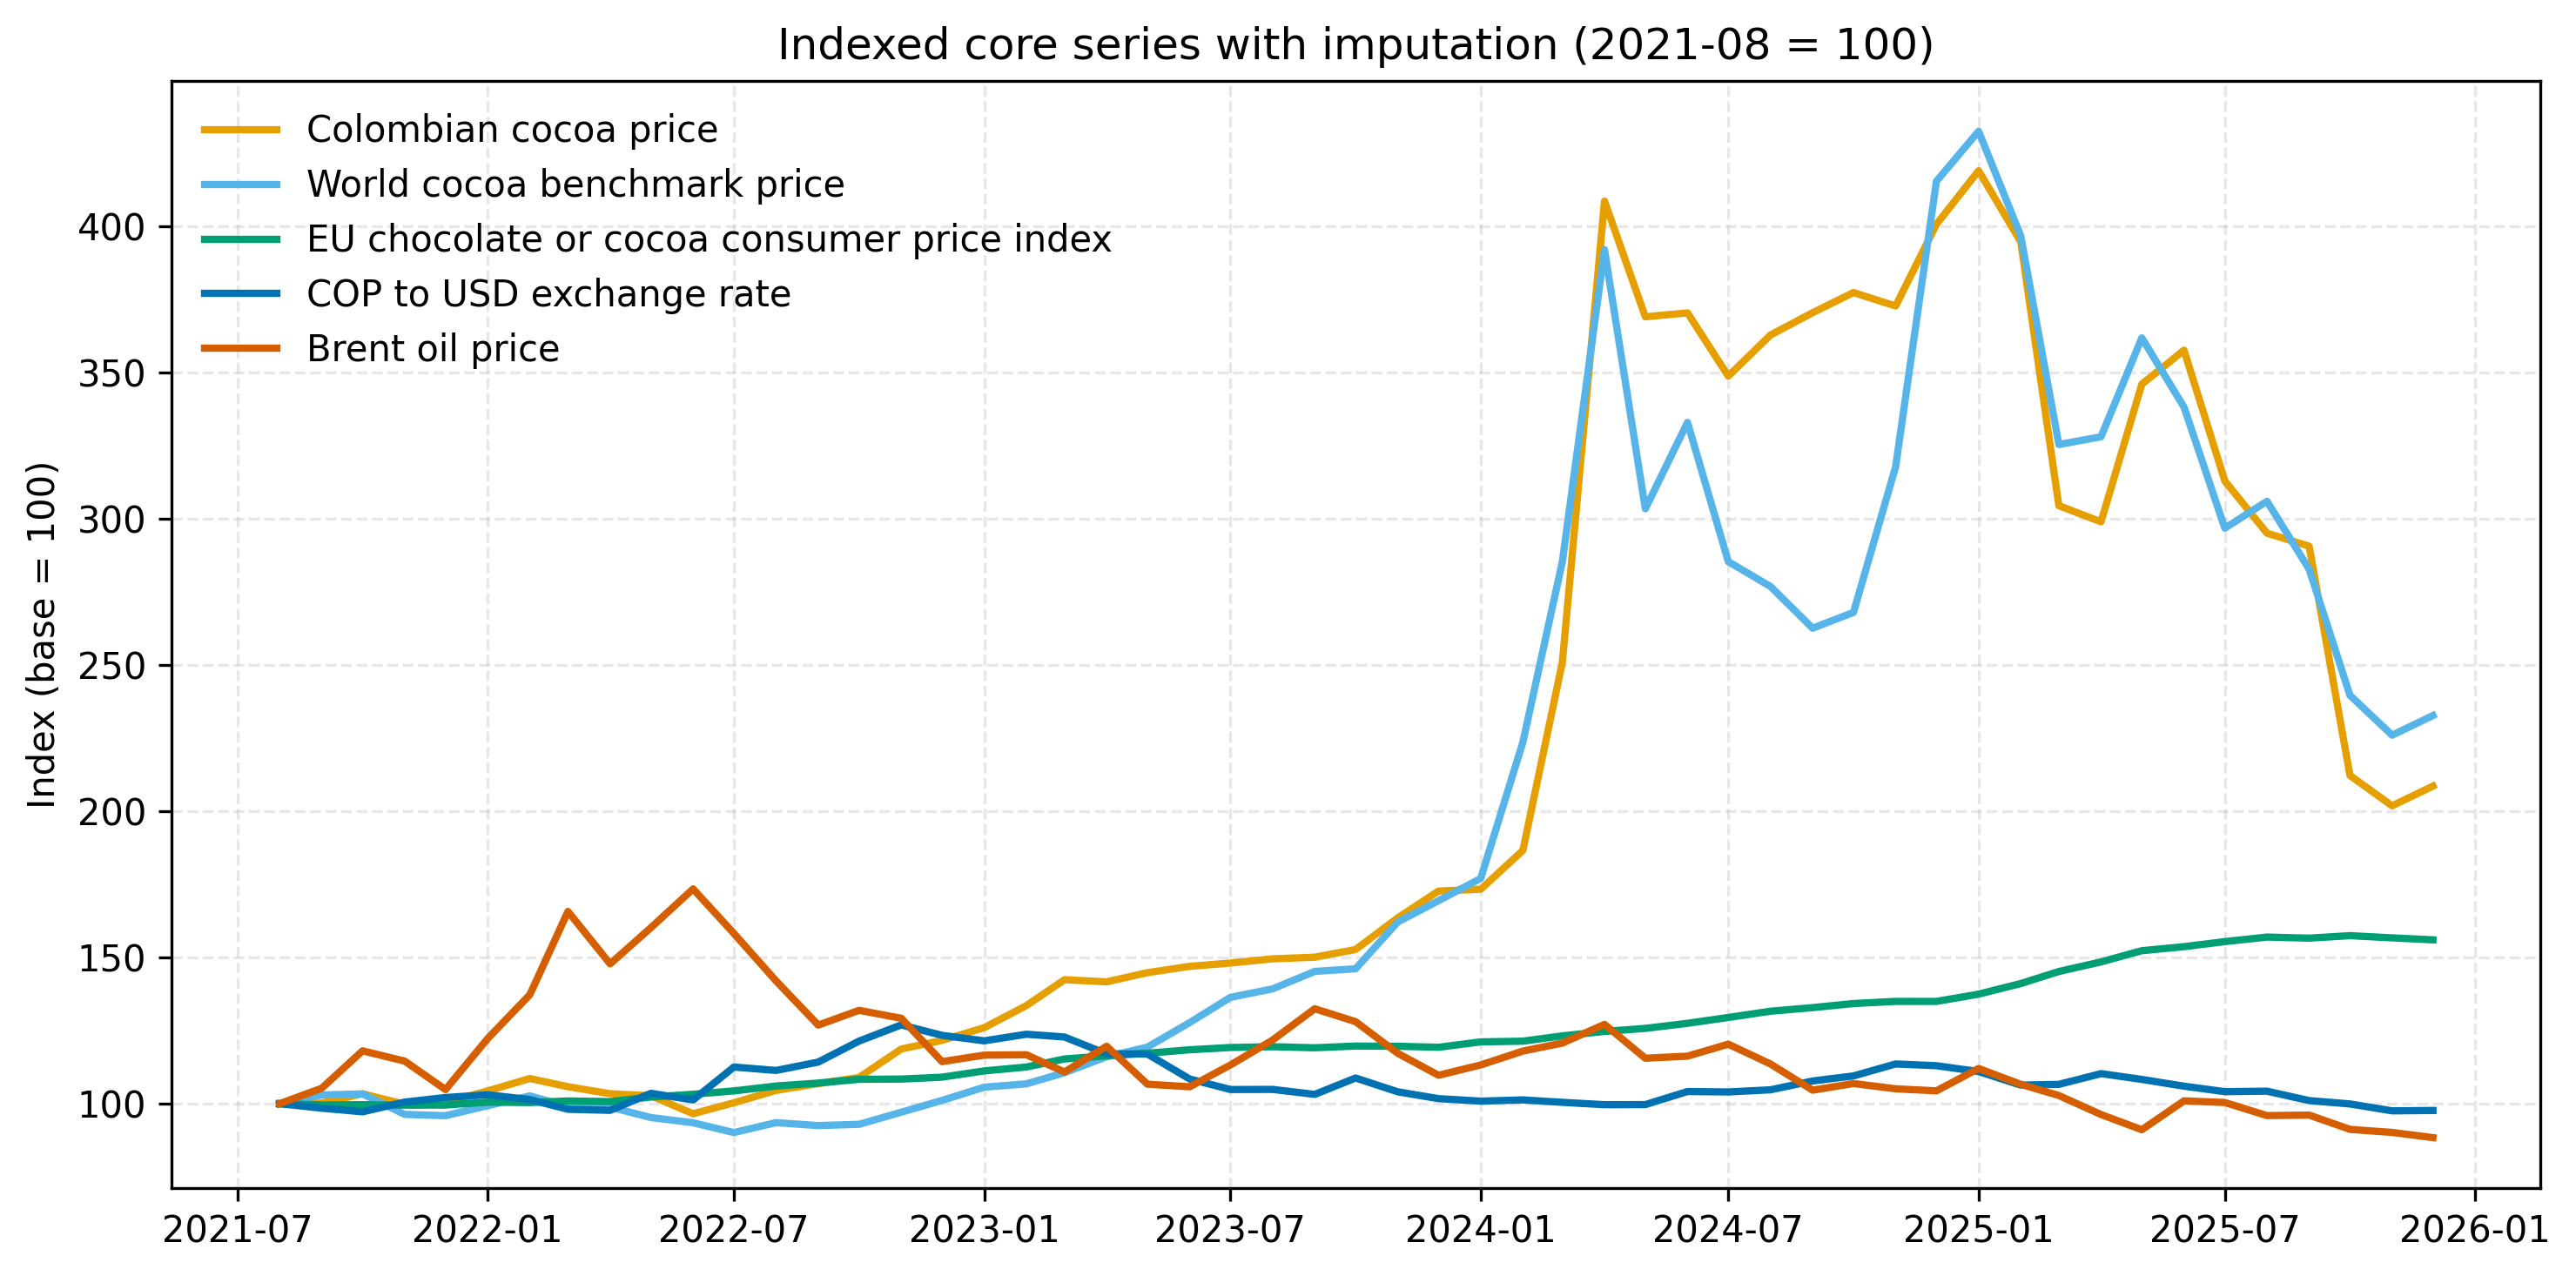
\includegraphics[width=0.95\textwidth]{figures/figure_indexed_core_series_common_window_imputed.png}
\caption{Indexed core series in the imputed shared monthly window. The figure compares proportional movements across Colombian cocoa, the world cocoa benchmark, the EU chocolate index, the exchange rate, and Brent oil in the common aligned sample.}
\label{fig:indexed_core}
\end{figure}

The common-window plot in Figure~\ref{fig:indexed_core} shows the close comovement between the Colombian and world cocoa series during the aligned period, alongside the smoother evolution of the EU downstream index. The same descriptive stage also reports a level correlation of 0.961 between Colombian cocoa and world cocoa and a log-return correlation of 0.730 between the same pair in the aligned sample.

\begin{figure}[H]
\centering
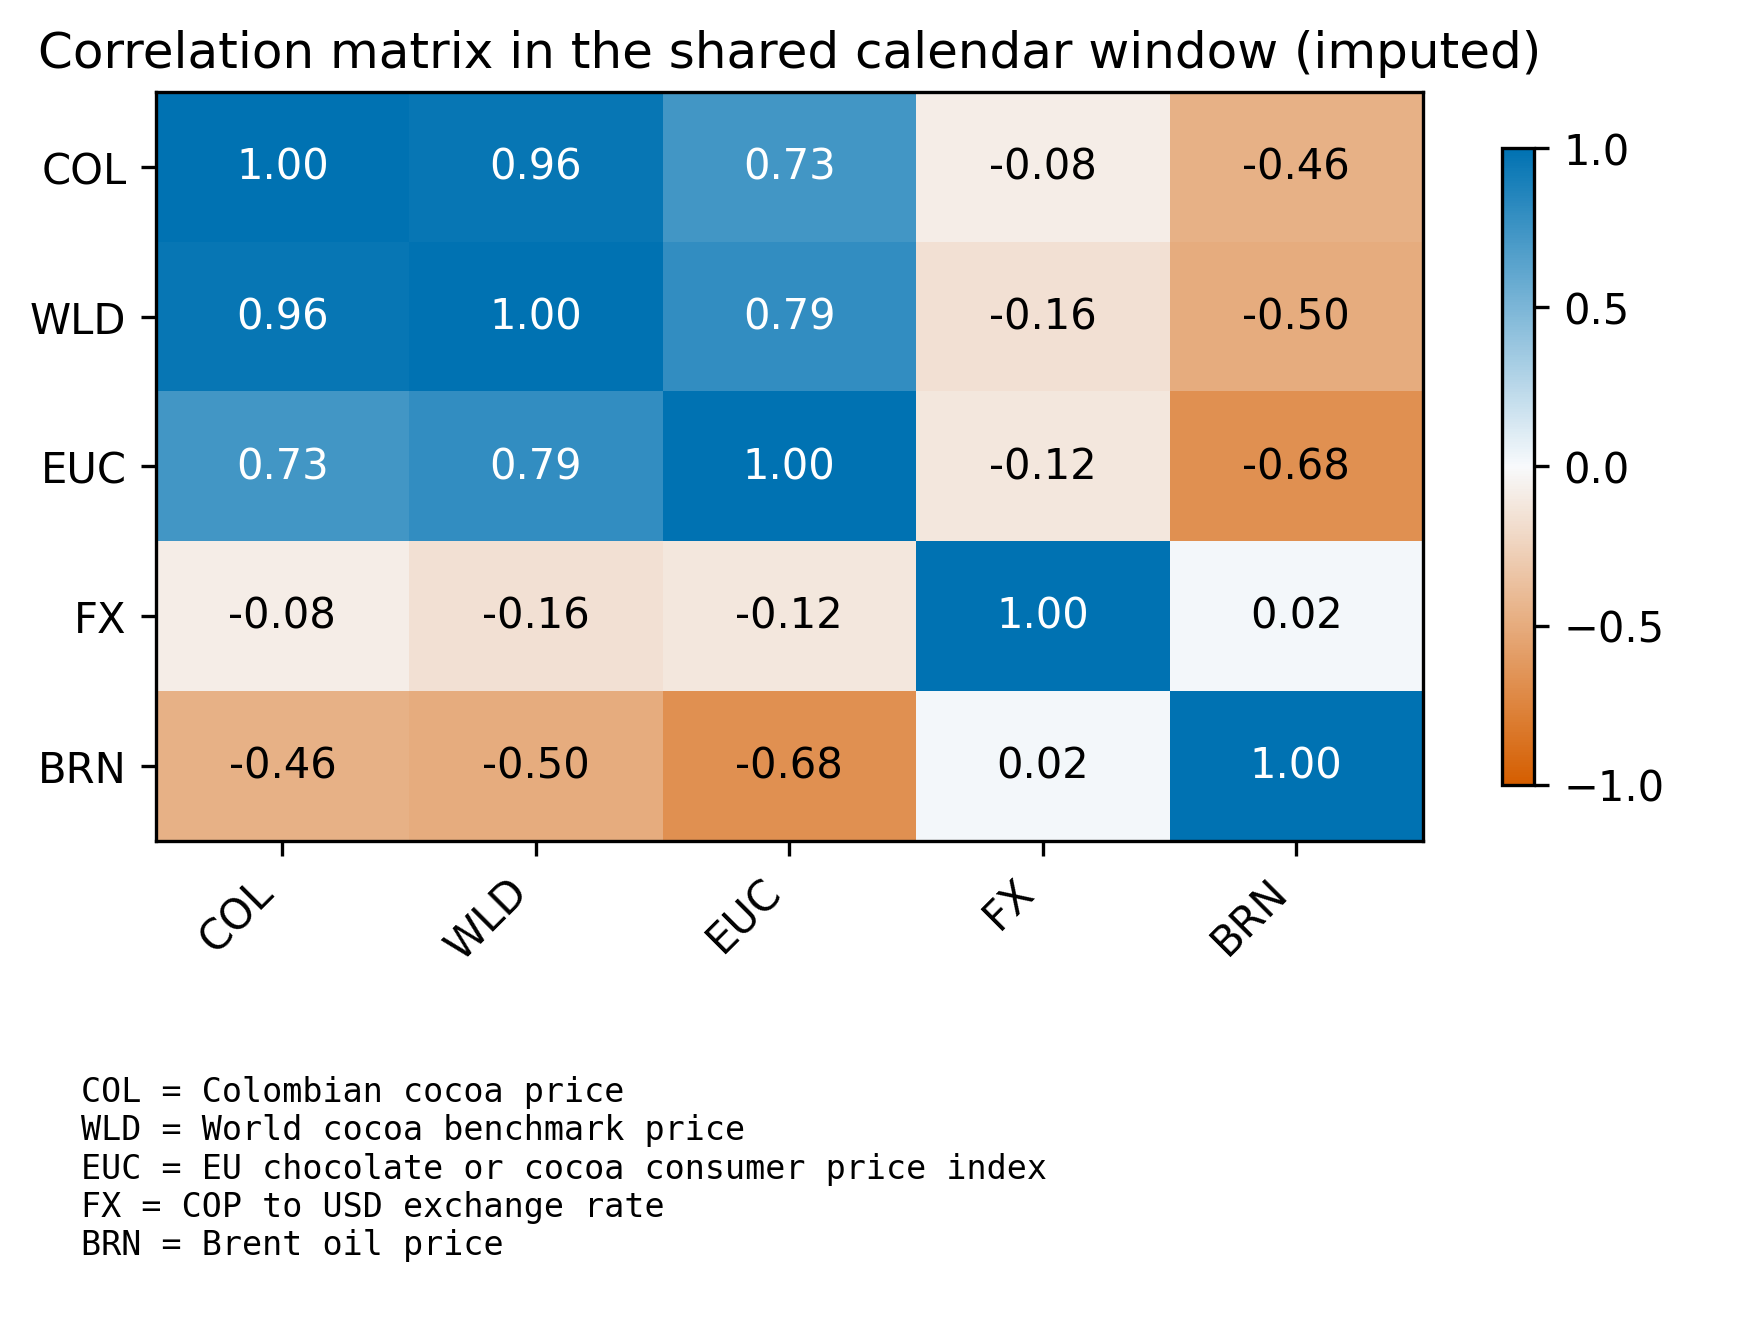
\includegraphics[width=0.90\textwidth]{figures/figure_correlation_heatmap_levels_common_window_imputed.png}
\caption{Correlation heatmap for the imputed aligned core system. The strongest relationship is between Colombian cocoa and the world cocoa benchmark, while the exchange rate is weakly associated with the price system in levels over the shared window.}
\label{fig:core_corrplot}
\end{figure}

Figure~\ref{fig:core_corrplot} makes the core dependence structure explicit. Colombian cocoa and world cocoa are highly correlated at the level ($0.961$), and both are positively associated with the EU chocolate index. Brent is negatively correlated with the three price indicators in the shared window, while COP/USD is comparatively weak in simple level correlation even though it remains important in the regression-based transmission equations.

\subsection{Preliminary Core Transmission Results}

The baseline transmission chapter provides the strongest evidence in the current draft. In the imputed long-run domestic-price equation, the elasticity on the world cocoa benchmark is 0.990, while the coefficient on the exchange rate is 0.902. In the short-run domestic-return equation, the world cocoa return coefficient is 0.796 with $p<0.001$, whereas the exchange-rate and Brent return coefficients are not conventionally significant. The model fit remains substantial, with adjusted $R^2=0.965$ for the level equation and adjusted $R^2=0.581$ for the domestic return equation. For the downstream EU series, the evidence is weaker: the level association with the world benchmark is positive, but the short-run return coefficient is small, negative, and estimated in a very low-fit equation. The downstream block therefore supports only a cautious interpretation of slower and weaker adjustment relative to the Colombian series.
\begin{table}[H]
\centering
\caption{Core transmission results from the imputed aligned sample}
\label{tab:core_results}
\small
\begin{tabular}{p{5.1cm}rrrr}
\toprule
Model component & Coefficient & Std. error & $p$-value & Adj. $R^2$ \\
\midrule
$\ln(P^{COL}_{t}) \leftarrow \ln(P^{WLD}_{t})$ & 0.990 & 0.037 & $<0.001$ & 0.965 \\
$\ln(P^{COL}_{t}) \leftarrow \ln(FX_t)$ & 0.902 & 0.147 & $<0.001$ & 0.965 \\
$\ln(P^{COL}_{t}) \leftarrow \ln(OIL_t)$ & 0.140 & 0.084 & 0.096 & 0.965 \\
$\Delta \ln(P^{COL}_{t}) \leftarrow \Delta \ln(P^{WLD}_{t})$ & 0.796 & 0.180 & $<0.001$ & 0.581 \\
$\Delta \ln(P^{COL}_{t}) \leftarrow \Delta \ln(FX_t)$ & 0.218 & 0.204 & 0.287 & 0.581 \\
$\Delta \ln(P^{COL}_{t}) \leftarrow \Delta \ln(OIL_t)$ & 0.029 & 0.067 & 0.665 & 0.581 \\
$\ln(P^{EU}_{t}) \leftarrow \ln(P^{WLD}_{t})$ & 0.296 & 0.126 & 0.018 & 0.727 \\
$\Delta \ln(P^{EU}_{t}) \leftarrow \Delta \ln(P^{WLD}_{t})$ & -0.023 & 0.010 & 0.023 & -0.007 \\
\bottomrule
\end{tabular}
\normalsize
\end{table}



\begin{table}[H]
\centering
\caption{Lag-specific pairwise Granger-causality $p$-values in the imputed aligned core return system}
\label{tab:granger_pvalues}
\small
\begin{tabular}{p{4.6cm}rrrr}
\toprule
Direction & Lag 1 $p$ & Lag 2 $p$ & Lag 3 $p$ & Best lag ($p$) \\
\midrule
World cocoa $\rightarrow$ Colombian cocoa & 0.050 & 0.075 & 0.023 & 3 (0.023) \\
Colombian cocoa $\rightarrow$ World cocoa & 0.013 & 0.076 & 0.027 & 1 (0.013) \\
Colombian cocoa $\rightarrow$ EU chocolate & 0.979 & 0.801 & 0.871 & 2 (0.801) \\
EU chocolate $\rightarrow$ Colombian cocoa & 0.692 & 0.781 & 0.641 & 3 (0.641) \\
World cocoa $\rightarrow$ EU chocolate & 0.678 & 0.597 & 0.364 & 3 (0.364) \\
EU chocolate $\rightarrow$ World cocoa & 0.866 & 0.191 & 0.192 & 2 (0.191) \\
\bottomrule
\end{tabular}
\normalsize
\end{table}



The cointegration and causality diagnostics support a cautious interpretation of the core transmission results. The bivariate Engle--Granger test for world cocoa and Colombian cocoa does not reject the null of no cointegration in the imputed aligned sample ($p=0.132$). Table~\ref{tab:granger_pvalues} reports the lag-specific Granger evidence. The strongest predictive linkage is from world cocoa returns to Colombian cocoa returns at lag 3 ($p=0.023$), but the reverse Colombia-to-world pairwise test is also significant at lags 1 and 3. In a short reduced-form sample, these results should be read as predictive precedence rather than as structural proof that domestic prices drive the world benchmark. Taken together with the regression elasticities and the impulse-response evidence, the results still support a world-to-Colombia transmission interpretation more strongly than the reverse.

\begin{figure}[H]
\centering
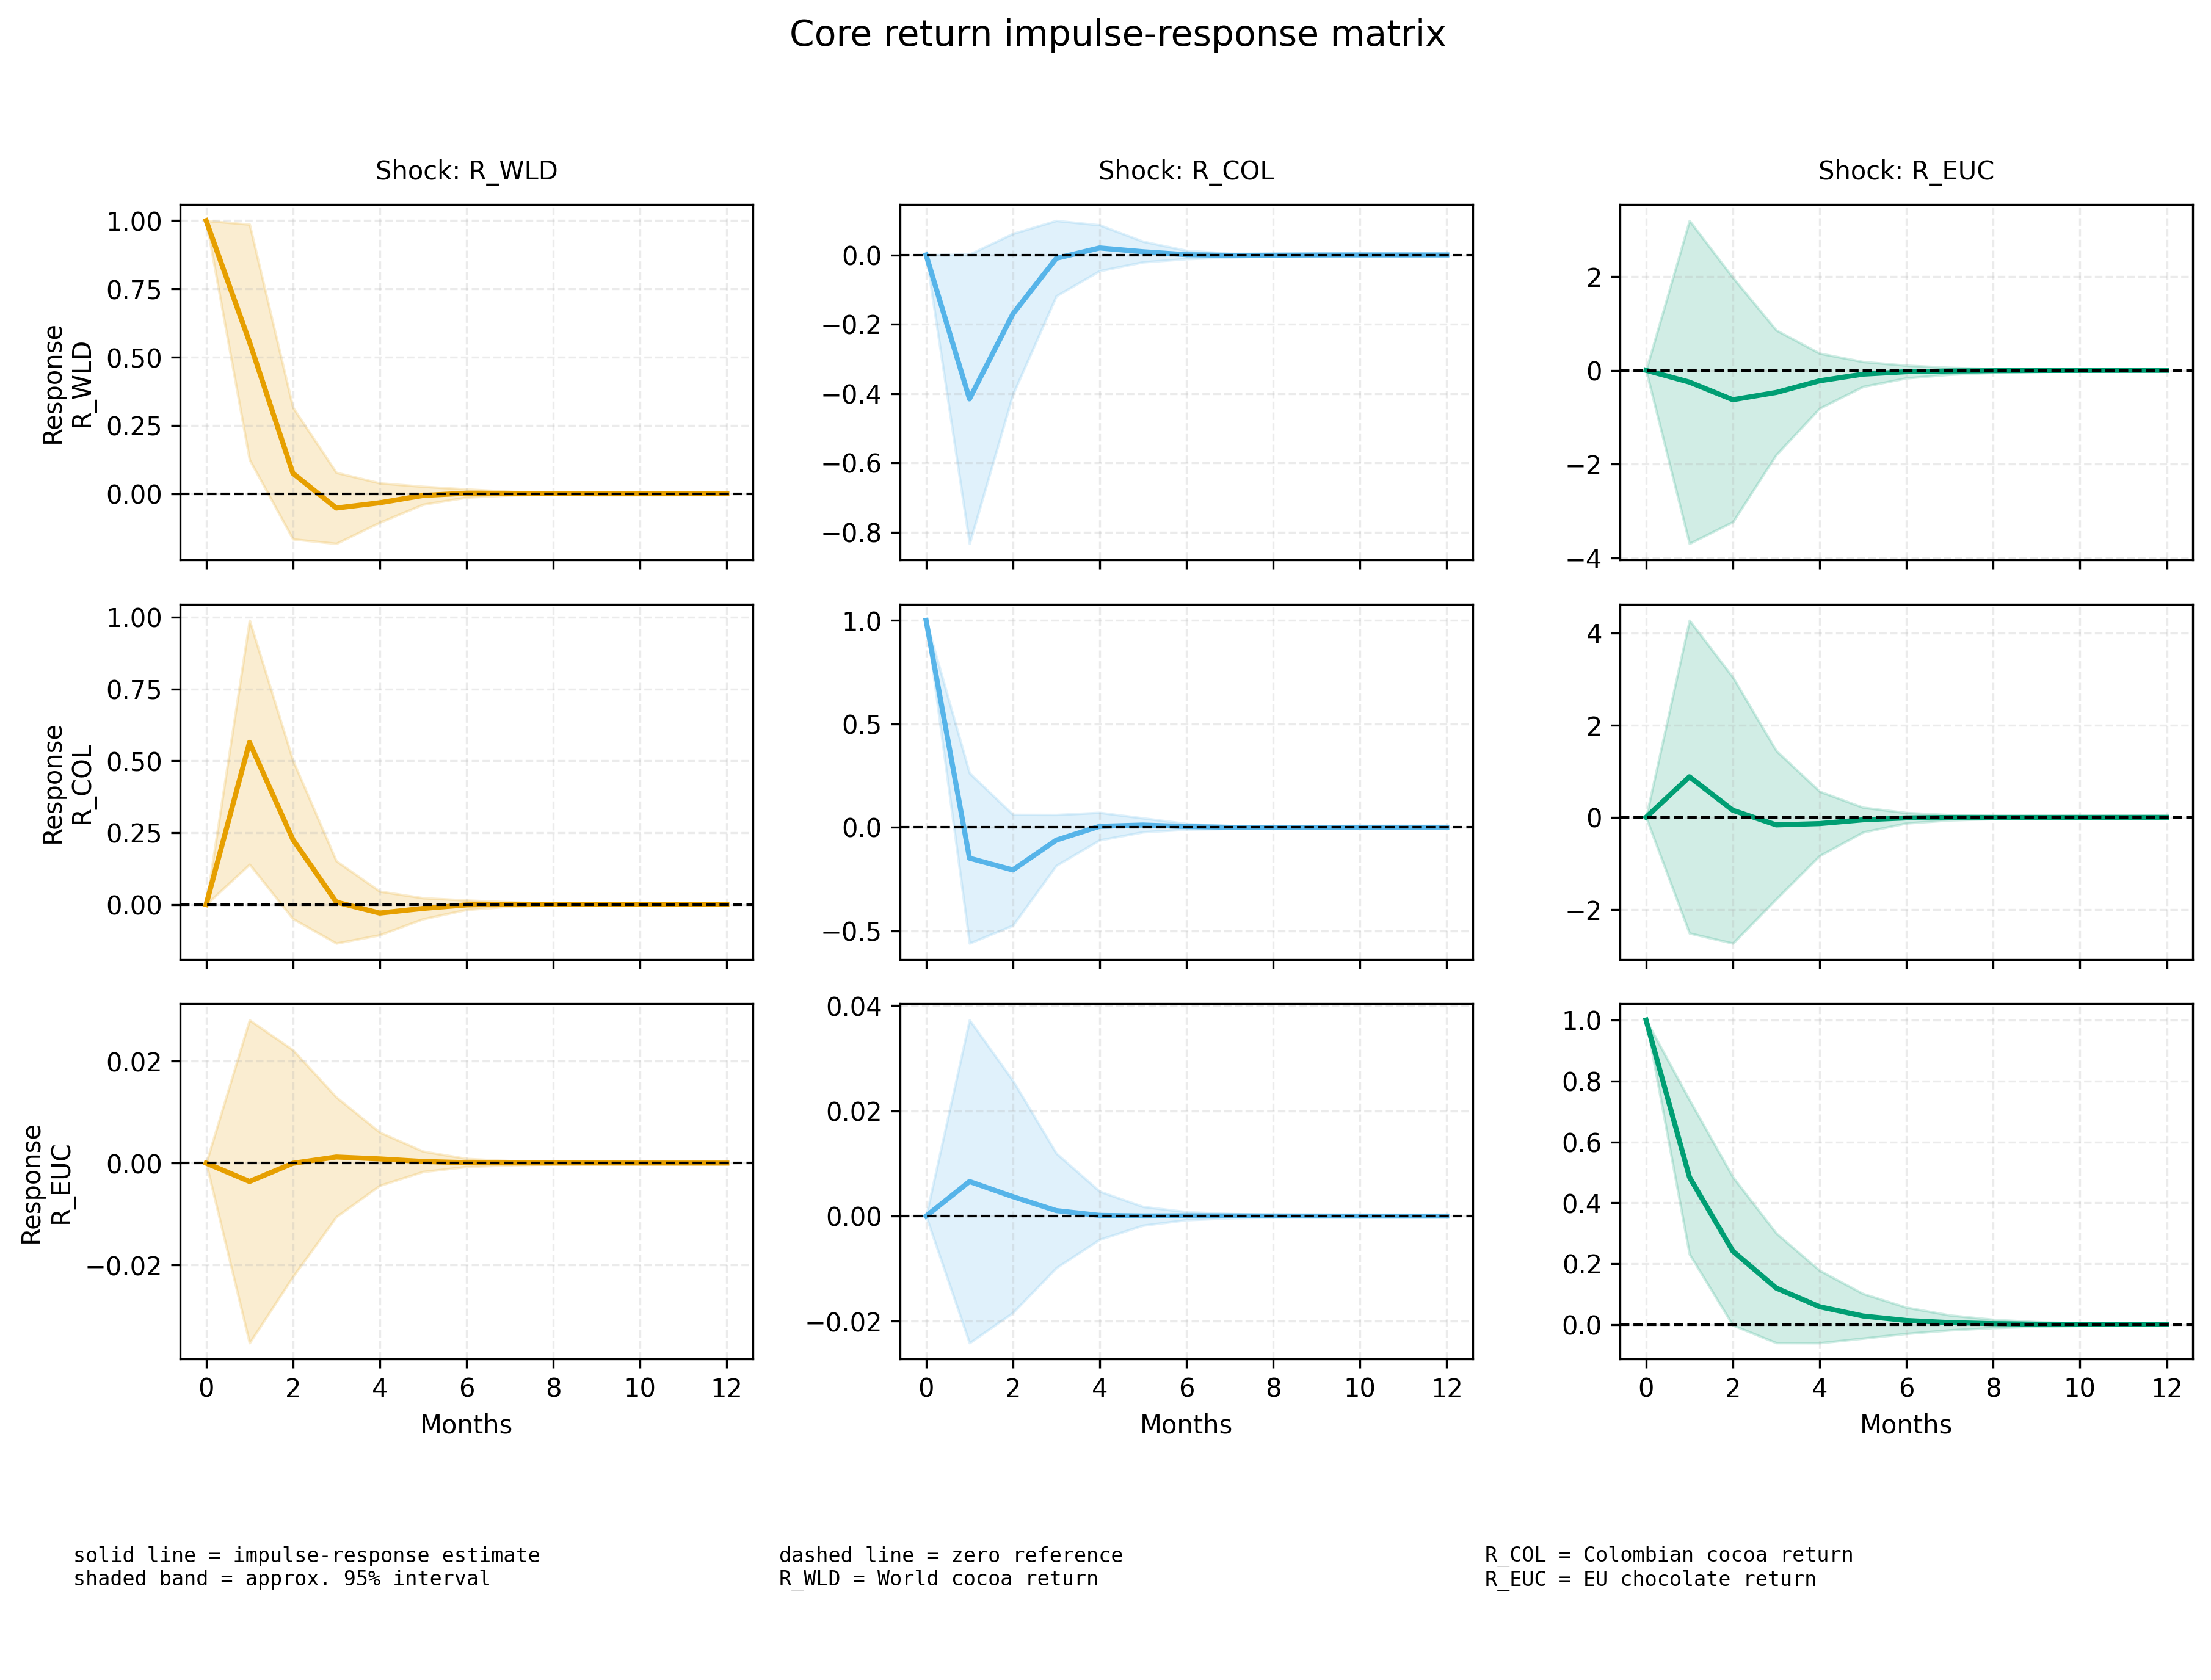
\includegraphics[width=\textwidth]{figures/figure_core_return_impulse_response.png}
\caption{Impulse-response matrix for the core return VAR. Acronyms identify the return series for world cocoa, Colombian cocoa, and the EU chocolate index.}
\label{fig:irf}
\end{figure}

\subsection{Preliminary Weather-Extended Results}

The weather chapter asks a different question. It does not ask whether local weather replaces market transmission. It asks whether local weather stress helps explain how market volatility is experienced in the producing location. The selected weather variables are precipitation, solar radiation, and maximum temperature. This choice follows the broader local cocoa weather architecture used in San Vicente de Chucur\'{\i} \citep{talero_sarmiento_etal_2025} and provides a parsimonious representation of water, radiation, and heat conditions in the aligned sample, while direct cocoa physiology support is strongest for the water- and heat-stress components \citep{Lahive2019}.

\begin{figure}[H]
\centering
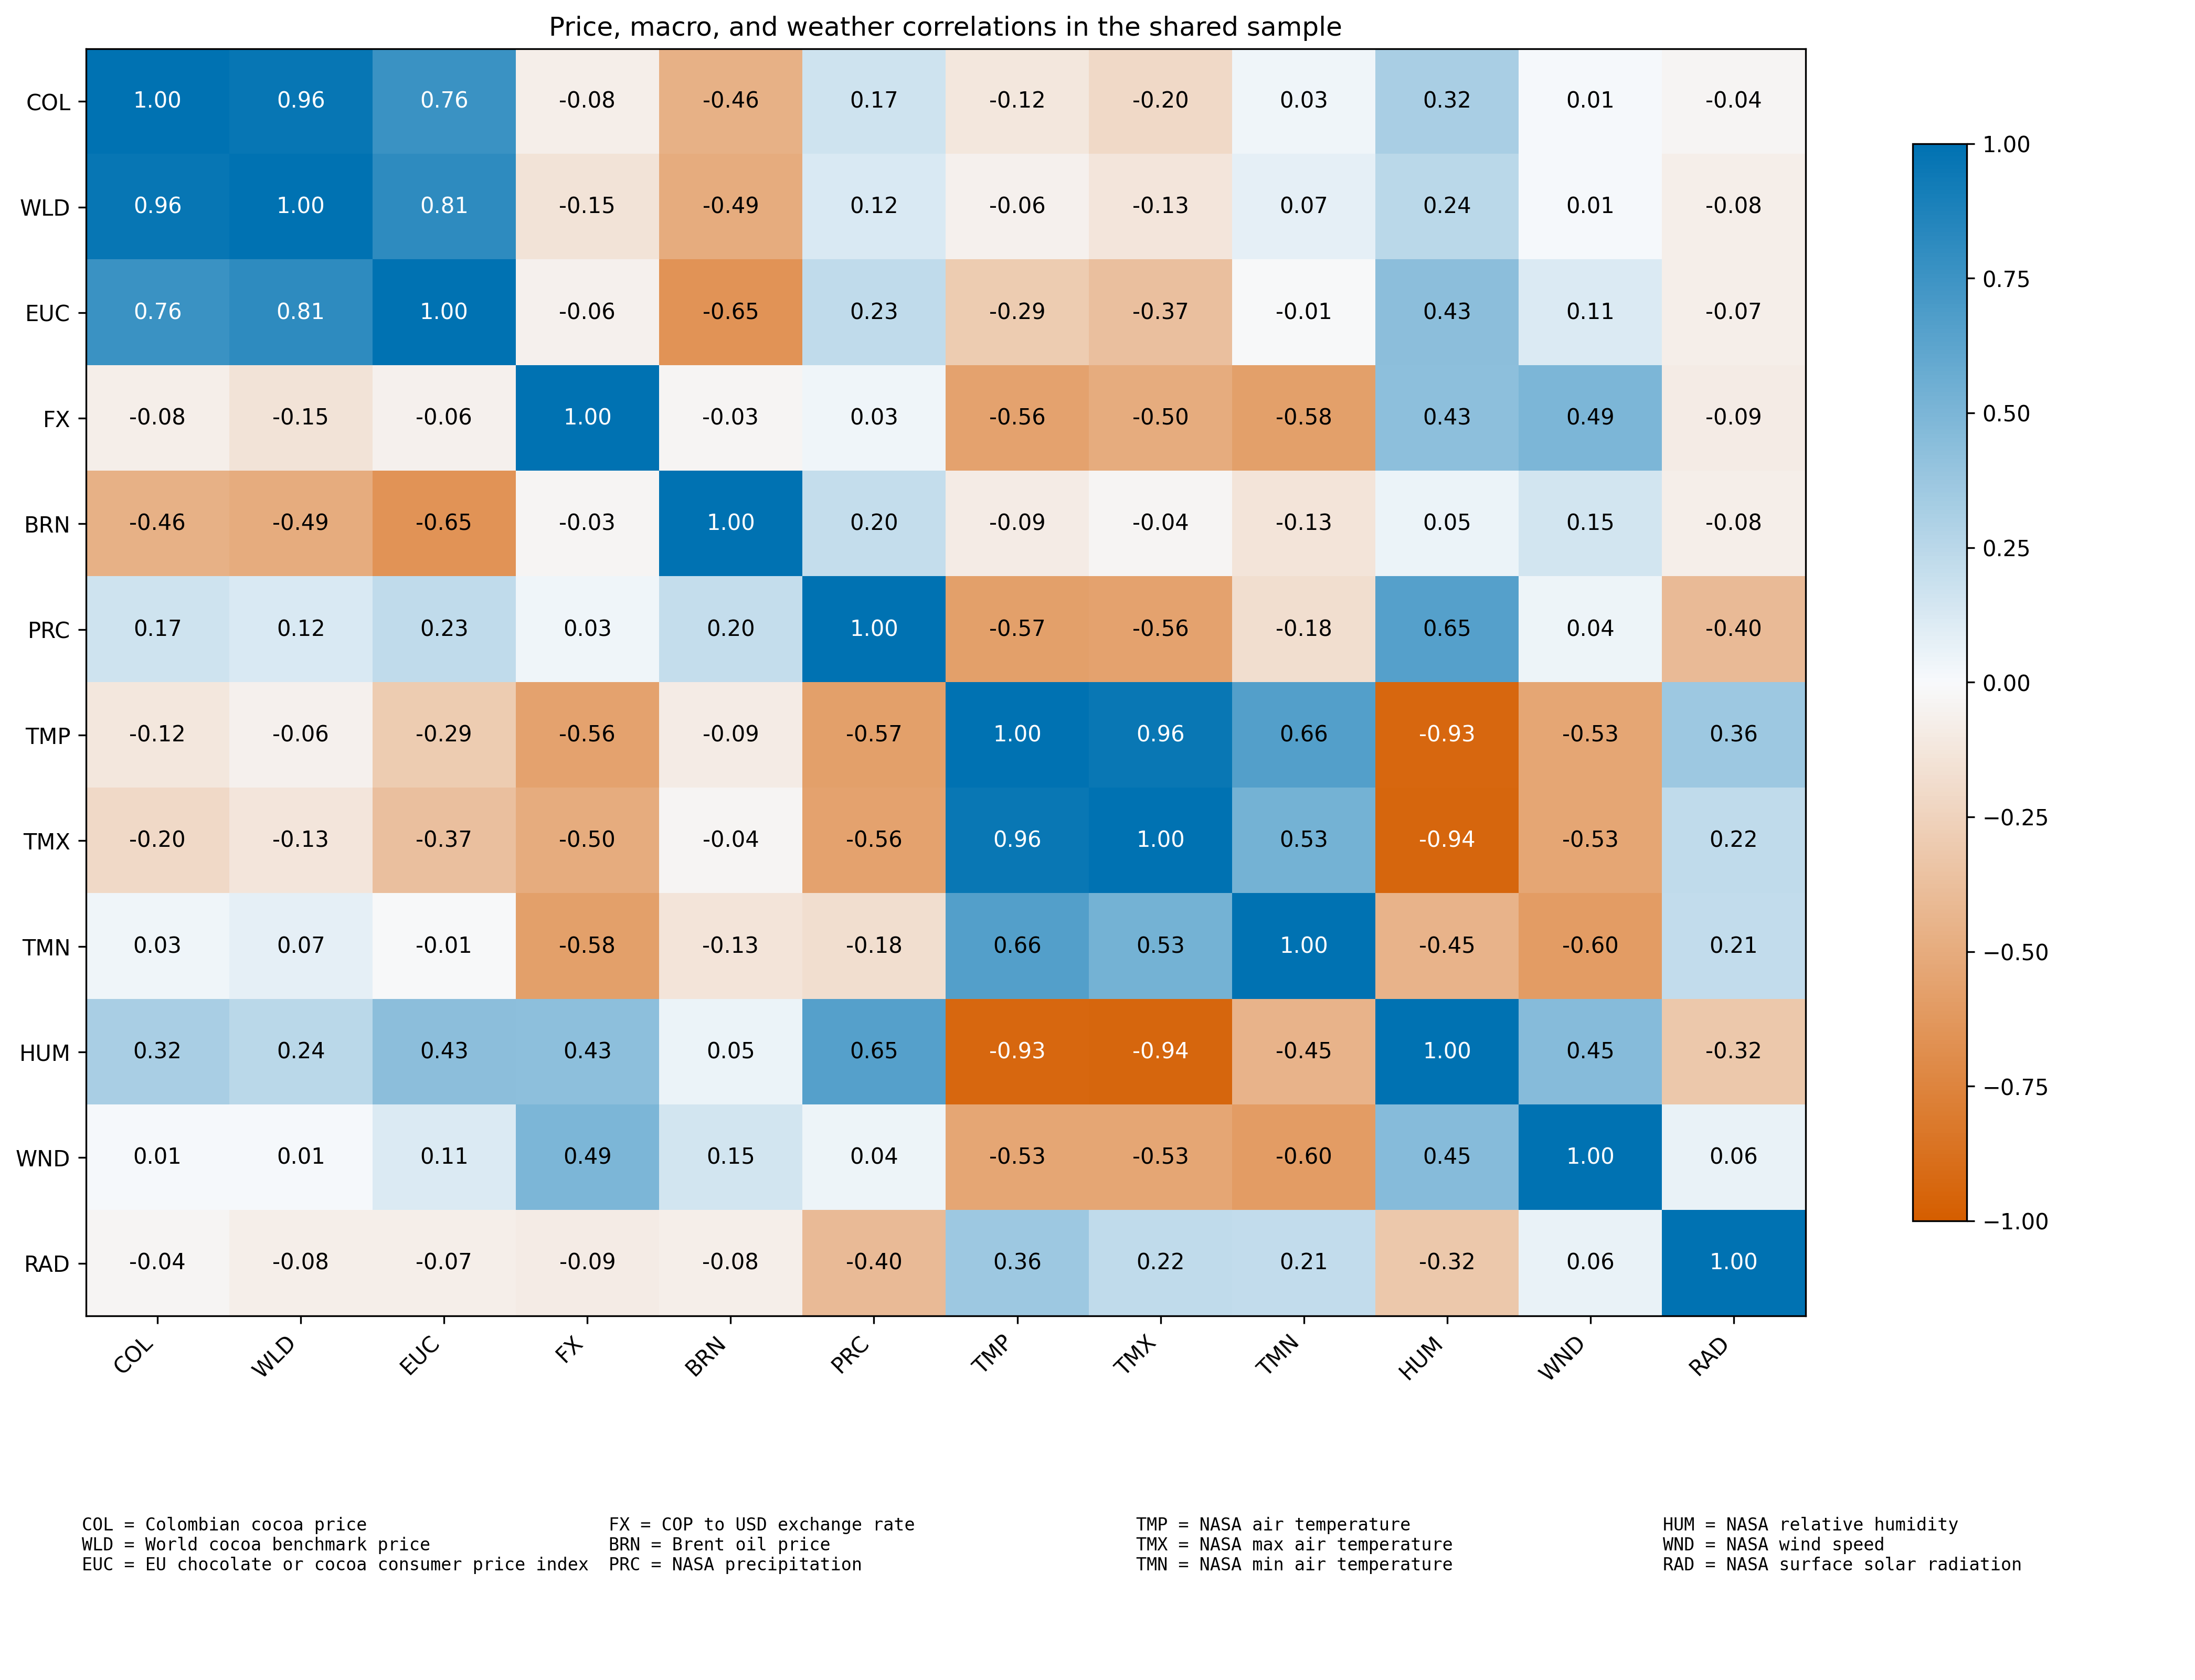
\includegraphics[width=\textwidth]{figures/figure_climate_core_correlation_common_sample.png}
\caption{Climate-core correlation matrix in the aligned common sample. This figure plays a parallel role to the impulse-response matrix for the core transmission block: it summarizes how the selected weather variables and the broader climate block relate to the price system without forcing an unstable weather-augmented VAR in a 51-observation complete sample.}
\label{fig:weather_corrplot}
\end{figure}

Figure~\ref{fig:weather_corrplot} is included because the second block is not currently estimated as a full weather-augmented VAR or VECM. Under the current climate-augmented overlap, such a system would be too parameter-heavy for defensible impulse-response analysis. The corrplot, therefore, provides a visual bridge between the weather data and the vulnerability interpretation. It shows, for example, that humidity is positively associated with the three price variables in the aligned sample, while temperature variables are negatively associated with the EU chocolate index and weakly to moderately associated with the core market variables.

\begin{figure}[H]
\centering
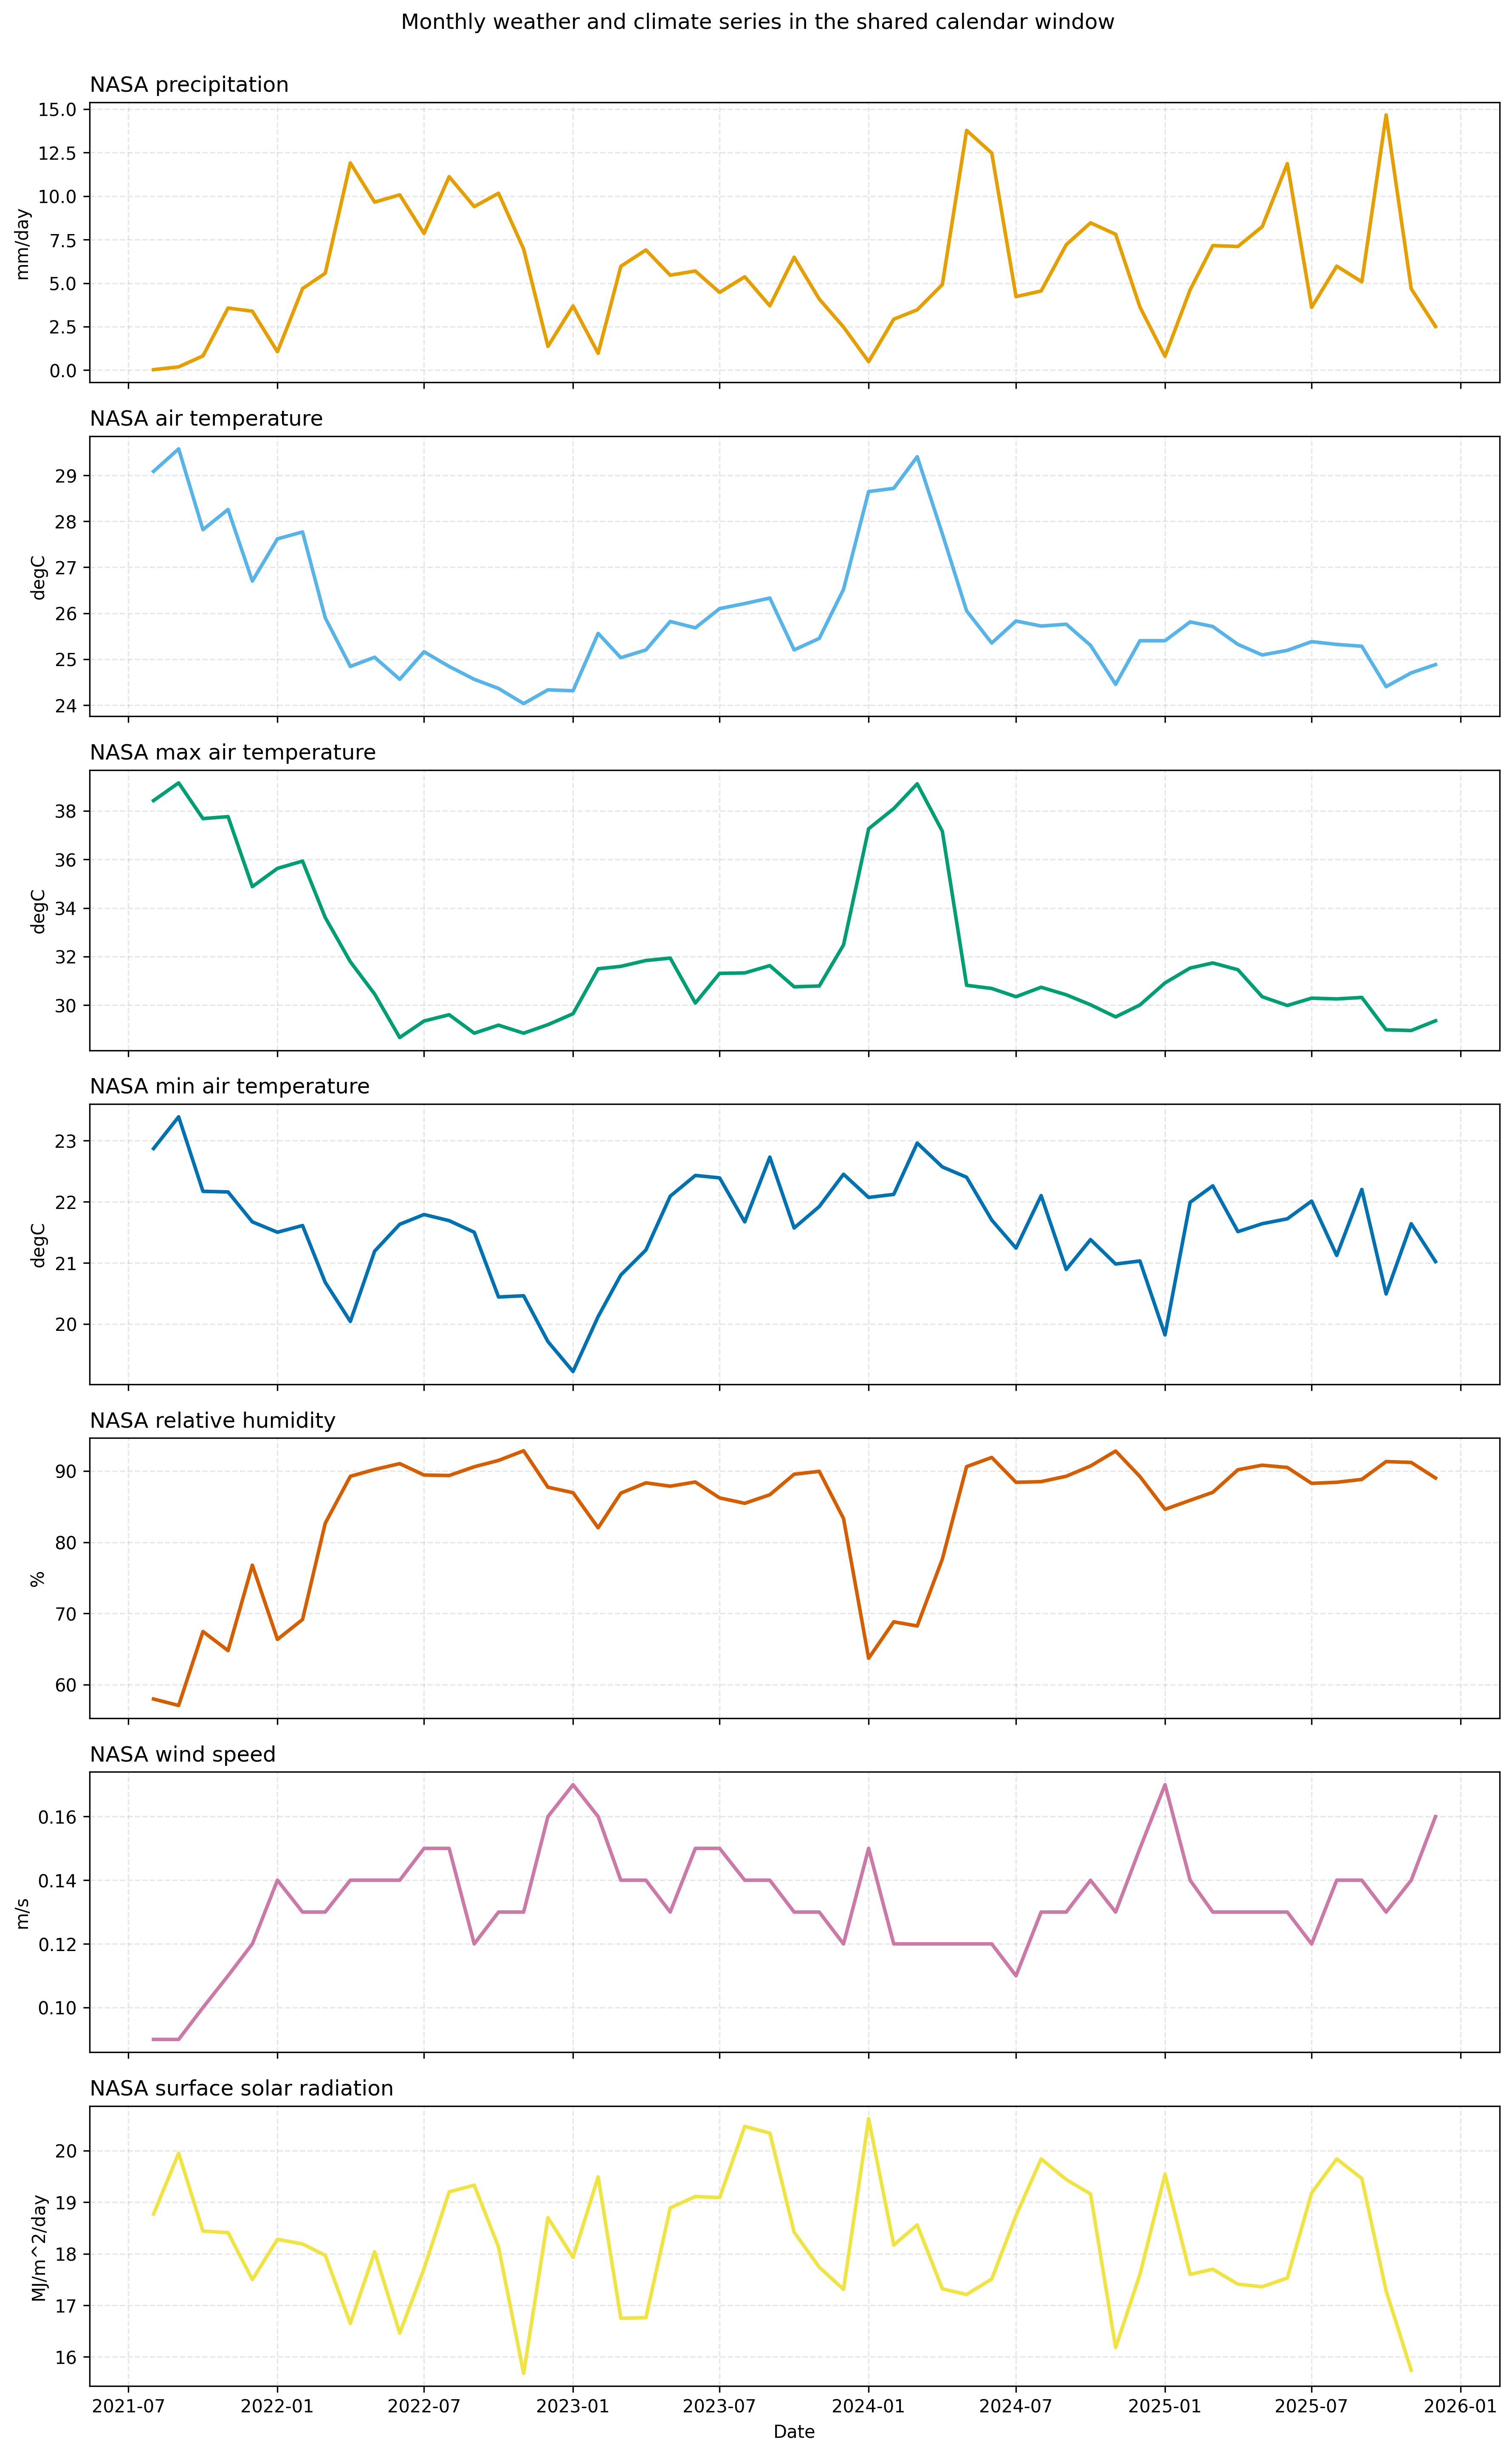
\includegraphics[width=\textwidth,height=0.82\textheight,keepaspectratio]{figures/figure_climate_series_panels_common_window.png}
\caption{Weather panels for the aligned common window in San Vicente de Chucur\'{\i}, Santander. These series provide the empirical context for the vulnerability chapter and for the exploratory climate-augmented approach.}
\label{fig:climate_panels}
\end{figure}
\begin{table}[H]
\centering
\caption{Weather-extended domestic models from the imputed aligned sample}
\label{tab:weather_results}
\small
\begin{tabular}{p{5.3cm}rrrr}
\toprule
Model component & Coefficient & Std. error & $p$-value & Adj. $R^2$ \\
\midrule
$\ln(P^{COL}_{t}) \leftarrow \ln(P^{WLD}_{t})$ & 0.977 & 0.037 & $<0.001$ & 0.966 \\
$\ln(P^{COL}_{t}) \leftarrow$ solar radiation$_t$ ($z$) & 0.028 & 0.016 & 0.075 & 0.966 \\
$\ln(P^{COL}_{t}) \leftarrow$ precipitation$_t$ ($z$) & 0.024 & 0.020 & 0.247 & 0.966 \\
$\ln(P^{COL}_{t}) \leftarrow$ max temperature$_t$ ($z$) & -0.009 & 0.019 & 0.627 & 0.966 \\
$\Delta \ln(P^{COL}_{t}) \leftarrow \Delta \ln(P^{WLD}_{t})$ & 0.773 & 0.157 & $<0.001$ & 0.595 \\
$\Delta \ln(P^{COL}_{t}) \leftarrow$ max temperature$_{t-1}$ ($z$) & 0.023 & 0.015 & 0.119 & 0.595 \\
$\Delta \ln(P^{COL}_{t}) \leftarrow$ precipitation$_{t-1}$ ($z$) & 0.003 & 0.010 & 0.725 & 0.595 \\
$\Delta \ln(P^{COL}_{t}) \leftarrow$ solar radiation$_{t-1}$ ($z$) & -0.008 & 0.008 & 0.330 & 0.595 \\
Domestic rolling volatility $\leftarrow$ world rolling volatility & 0.954 & 0.051 & $<0.001$ & 0.917 \\
Domestic rolling volatility $\leftarrow$ weather stress$_{t-1}$ & 0.013 & 0.012 & 0.253 & 0.917 \\
\bottomrule
\end{tabular}
\normalsize
\end{table}

The weather extension improves adjusted $R^2$ only modestly relative to the core domestic models. The improvement is 0.0017 in levels and 0.0139 in returns, and most individual weather coefficients are not conventionally significant. This is still interpretively useful because it suggests that weather matters more for vulnerability framing than for replacing the benchmark market variables in the core transmission mechanism.
\begin{table}[H]
\centering
\caption{Definition and empirical range of the exploratory vulnerability indicators}
\label{tab:vulnerability_definitions}
\small
\begin{tabular}{p{3.0cm}p{8.2cm}rr}
\toprule
Indicator & Construction in the current draft & Mean & Std. dev. \\
\midrule
Weather stress index & Mean absolute standardized anomaly across precipitation, solar radiation, and maximum temperature & 0.798 & 0.356 \\
Weather stress ($z$-score) & Standardized weather-stress index; positive values indicate above-average combined weather anomaly in the aligned sample & 0.000 & 1.010 \\
Farmer exposure index & $z(\sigma^{COL}_t) + z(\widehat{m}_t) + \text{WeatherStressZ}_t$ & 0.758 & 1.691 \\
Livelihood risk score & $\text{FarmerExposureIndex}_t + z(\sigma^{WLD}_t)$ & 0.758 & 2.429 \\
\bottomrule
\end{tabular}
\normalsize
\end{table}


\begin{figure}[H]
\centering
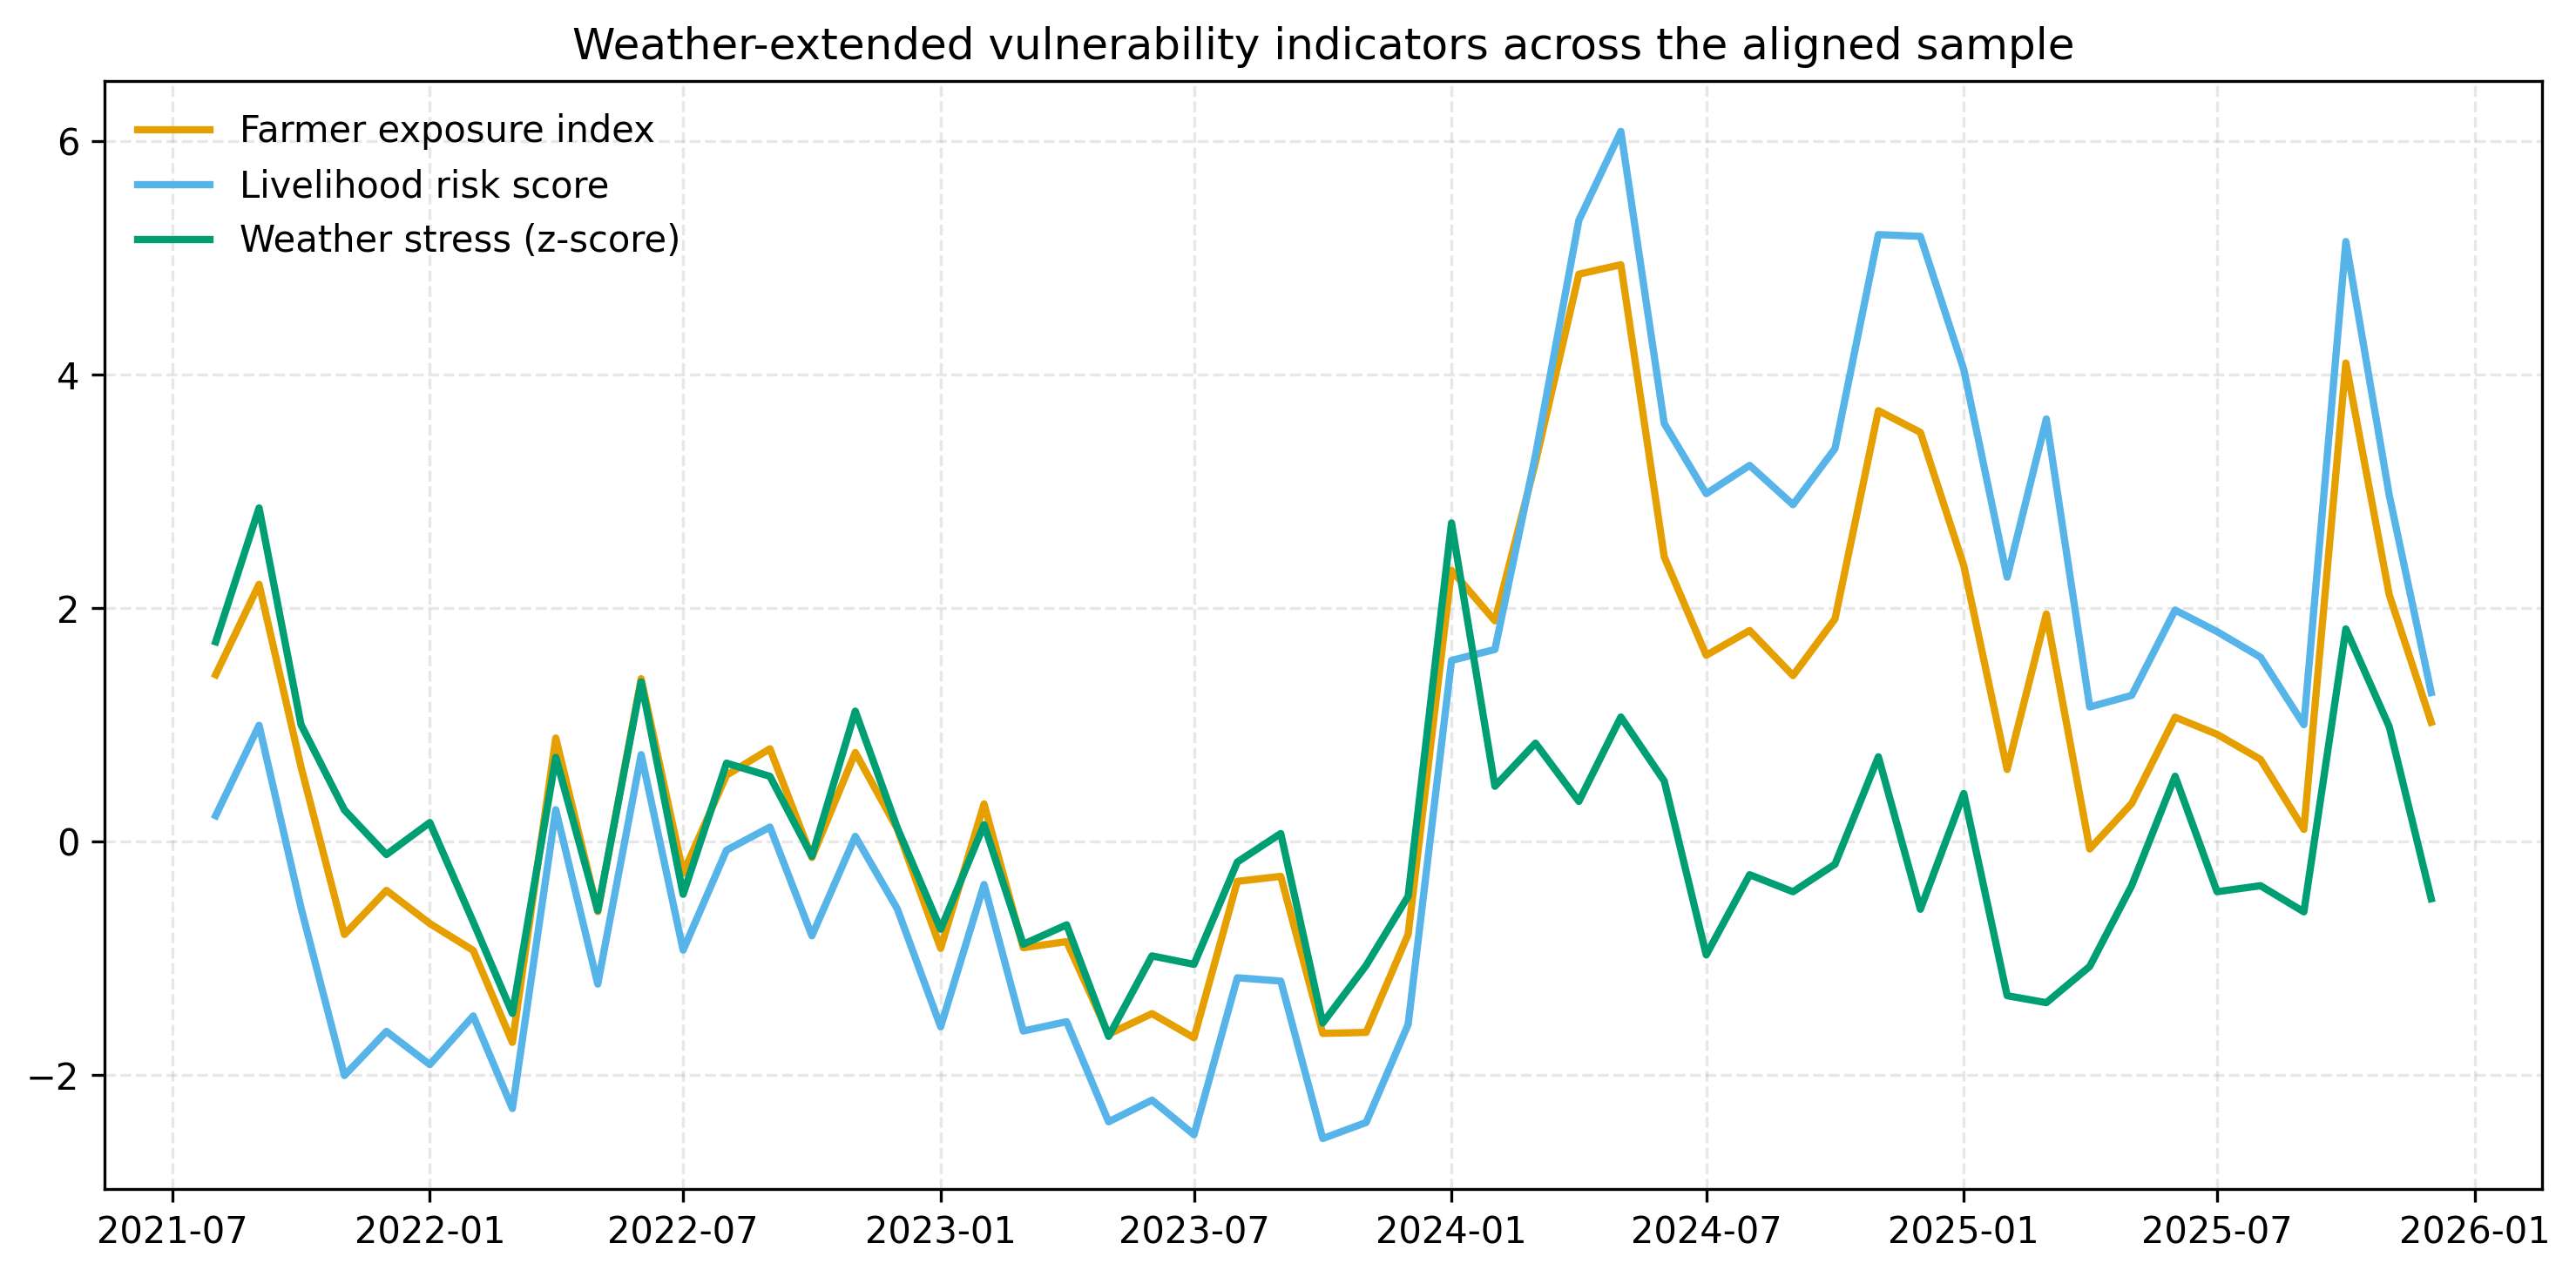
\includegraphics[width=0.93\textwidth]{figures/figure_weather_vulnerability_index.png}
\caption{Exploratory weather-extended vulnerability indicators. Weather stress ($z$-score) standardizes the average absolute anomaly across precipitation, solar radiation, and maximum temperature; the farmer exposure index adds domestic volatility and fitted market-transmission shock; the livelihood-risk score additionally incorporates world-cocoa volatility.}
\label{fig:vulnerability}
\end{figure}

Table~\ref{tab:vulnerability_definitions} and Figure~\ref{fig:vulnerability} clarify the meaning of the exploratory indicators. Weather stress is not a raw climate level; it is a relative anomaly score within the aligned sample. The farmer exposure index should therefore be read as a standardized combination of domestic volatility, predicted market-shock magnitude, and local weather anomaly. The livelihood-risk score adds world-cocoa volatility in order to represent an external market-pressure layer on top of local exposure. The highest-risk months under this exploratory scoring are May 2024, April 2024, November 2024, December 2024, and October 2025. These dates should be interpreted as descriptive outputs of the exploratory index rather than as validated welfare rankings, but they remain consistent with the broader idea that vulnerability in this system is produced by the interaction of transmitted market shocks and local stress conditions, not by weather alone.

\subsection{Preliminary Answers to the Gap Questions and Hypotheses}

\textbf{Gap question 1 / H1 is supported.} The clearest result in the draft is the positive and statistically strong effect of world cocoa returns on Colombian cocoa returns.

\textbf{Gap questions 1--2 / H2 is partially supported.} The EU downstream series moves with the system in levels, but the short-run return response is much weaker and the EU return model has poor fit.

\textbf{Gap question 3 / H3 is partially supported.} Weather variables do not dominate the market system, but they do improve the vulnerability narrative and contribute modestly to model fit, especially through solar radiation in levels and heat stress in lagged returns.

\textbf{Gap question 3 / H4 is provisionally supported.} The climate-augmented system remains theoretically attractive but empirically fragile under the current 51-observation complete weather overlap. For now, the manuscript should emphasize weather as contextual vulnerability information and present climate-augmented cointegration as an exploratory extension rather than as the main result.

\section{Discussion}
\label{sec:discussion}

This manuscript set out to address a specific gap in the cocoa literature: the limited number of empirical designs that trace how benchmark commodity shocks reach producers while placing those shocks in local environmental context. The clearest finding is that international cocoa movements remain the dominant short-run driver of Colombian cocoa price changes in the aligned window. This matters because existing cocoa studies already document producer exposure to price volatility, weak farmer organizations, dependence on few buyers, and climate-related production risks \citep{Mithofer2017,AkrofiAtitianti2018}. The present results complement that evidence by identifying a concrete channel through which global instability becomes locally relevant for producers. Put differently, resilience in cocoa-producing territories cannot be assessed only through agronomy or governance indicators if the market-exposure mechanism is left unmeasured.

The second gap question concerned differential adjustment across the supply chain. Here the results are informative, but more qualified than in the domestic transmission block. Colombian producer-linked prices move closely with the world benchmark, whereas the EU chocolate index shows a positive level association but a much weaker and less stable short-run response. Taken together with the lower downstream volatility, this pattern is consistent with a cocoa-chain interpretation in which exposure is unevenly distributed across actors, but it should not be read as definitive proof of downstream buffering in a structural sense. Earlier cocoa studies similarly show that integration into world markets can increase farmer exposure without proportionate gains to farmers, while producer concerns remain shaped by weak organizations and dependence on limited market channels \citep{TsowouGayi2019,Mithofer2017}. Comparative work on coffee value chains points in the same general direction for tropical tree crops cultivated under similar conditions, emphasizing that adaptive capacity depends on support and coordination across the chain \citep{Morales2022,Verburg2019}. The manuscript cannot identify the exact institutional mechanism behind differential adjustment, but the results remain consistent with the idea that value-chain position matters for how shocks are absorbed or passed on.

The third gap question concerned the role of local weather stress. The weather block does not overturn the market results, and that negative finding is informative. Rather than showing that climate variables dominate short-run price formation, the estimates support a narrower and more defensible interpretation: local weather conditions help identify when transmitted market shocks are experienced under tighter environmental stress. This interpretation is strengthened more by the conceptual role of the weather block and the exploratory index construction than by strong standalone weather coefficients in the regressions. It is consistent with cocoa studies showing that vulnerability depends on climatic suitability, physiological sensitivity, farm management, and ecological design \citep{Schroth2016,Lahive2019}. It is also consistent with evidence that agroforestry and diversified systems can improve buffering capacity, income diversification, and adaptation potential under cocoa climate stress \citep{Jacobi2013,Niether2020,Vaast2014}. Comparable climate-risk work on coffee likewise suggests that adaptation support in perennial tropical cash crops has to be targeted to the regions and systems facing the highest environmental stress \citep{Koh2020,Laderach2016}. For that reason, the exploratory vulnerability indicators proposed here should be read as transparent organizing devices rather than as validated welfare measures.

These contributions should be interpreted alongside several limitations. The main limitation is sample length. The core aligned monthly window contains only 53 months, and the fully complete climate-augmented overlap contains only 51 months. This is sufficient for transparent descriptive work and cautious reduced-form analysis, but it is short for strong multivariate cointegration claims in a system that mixes domestic, benchmark, downstream, macro, and climate variables \citep{hakkio_rush_1991}. A second limitation is the structure of the missing-data problem. Although only two cells required imputation, any imputed value remains an estimate rather than a recovered observation. The manuscript therefore treats imputation as a continuity device and a sensitivity tool, not as a remedy for fundamental data scarcity.

Measurement also constrains the scope of inference. The Colombian domestic series is a national weekly reference price aggregated to monthly means, not a farm-gate micro panel; the EU downstream series is a consumer-price index rather than a wholesale chocolate margin; and the weather block is a location-level NASA POWER panel rather than a farm-observed yield or disease dataset. These features do not invalidate the analysis, but they mean that the paper is strongest when it speaks about transmission, volatility, and vulnerability context across linked market layers rather than about farm-level agronomic causality. The manuscript also inherits institutional source transitions, particularly the legacy Eurostat COICOP endpoint through December 2025 and the March 2026 Brent extension derived from official daily data. These issues are documented for replication, but they still matter for future updating.

Even with those constraints, the paper contributes to both theory and policy. Conceptually, it argues for treating resilience in commodity systems as an interaction between transmitted market instability and local adaptive context rather than as a purely ecological, institutional, or behavioral attribute in isolation, consistent with vulnerability and food-system resilience frameworks \citep{Turner2003,Adger2006,Zurek2022}. Empirically, it shows that a transparent transmission design can make that interaction visible even before household microdata are available. For policy, the implication is that producer resilience cannot be assessed through climate adaptation measures alone. The current evidence most strongly supports benchmark pass-through, the broader macroeconomic environment in which transmission occurs, differences in adjustment across market layers, and locally weather-sensitive support systems as parts of the same diagnostic frame \citep{Gereffi2005,Merkle2021}.

\section{Conclusion}

This paper presents a transparent empirical framework for studying cocoa price volatility and smallholder vulnerability across the supply chain. Its main contribution is to address three questions within one design: how international cocoa shocks are transmitted to Colombian producer-linked prices once exchange-rate and oil conditions are considered, whether adjustment is distributed unevenly between producer-linked and downstream prices, and whether local weather should be interpreted as contextual stress rather than as the dominant short-run price driver.

The preliminary evidence points to three aligned conclusions. First, transmission from international cocoa markets to Colombian domestic prices is strong and statistically robust, indicating that producer exposure is closely tied to benchmark movements within a broader macroeconomic environment. Second, the European downstream chocolate index shows weaker and less stable short-run adjustment, which is consistent with, but does not by itself prove, uneven distribution of adjustment across actors in the supply chain. Third, the weather variables do not overturn the core transmission results, and their main value in the current draft is to identify the local stress context in which market-driven exposure is experienced.

Taken together, these results suggest that vulnerability in the cocoa chain is shaped by transmitted market instability, the macroeconomic setting of transmission, differences in adjustment across market layers, and local stress conditions. The paper therefore contributes to resilience research by showing that market transmission itself is part of the exposure mechanism that vulnerability analysis must explain \citep{Turner2003,Adger2006}. For policy, the implication is that producer resilience cannot be strengthened through climate adaptation measures alone; it also requires attention to benchmark pass-through and to the institutional conditions that determine how shocks are absorbed or passed along the chain \citep{Gereffi2005,Merkle2021}.

\bibliographystyle{apalike}
\bibliography{references/cocoa_volatility}

\end{document}
